%%%%%%%%%%%%%%%%%%%%%%%%%%%%%%%%%%%%%%%%%
% Short Sectioned Assignment LaTeX Template Version 1.0 (5/5/12)
% This template has been downloaded from: http://www.LaTeXTemplates.com
% Original author:  Frits Wenneker (http://www.howtotex.com)
% License: CC BY-NC-SA 3.0 (http://creativecommons.org/licenses/by-nc-sa/3.0/)
%%%%%%%%%%%%%%%%%%%%%%%%%%%%%%%%%%%%%%%%%

%----------------------------------------------------------------------------------------
%	PACKAGES AND OTHER DOCUMENT CONFIGURATIONS
%----------------------------------------------------------------------------------------

\documentclass[paper=a4, fontsize=11pt]{scrartcl} % A4 paper and 11pt font size

% ---- Entrada y salida de texto -----

\usepackage[T1]{fontenc} % Use 8-bit encoding that has 256 glyphs
\usepackage[utf8]{inputenc}
%\usepackage{fourier} % Use the Adobe Utopia font for the document - comment this line to return to the LaTeX default

% ---- Idioma --------

\usepackage[spanish, es-tabla]{babel} % Selecciona el español para palabras introducidas automáticamente, p.ej. "septiembre" en la fecha y especifica que se use la palabra Tabla en vez de Cuadro

% ---- Otros paquetes ----

\usepackage[hidelinks]{hyperref} % Estilo para los enlaces
\hypersetup{
  colorlinks   = true, %Colours links instead of ugly boxes
  urlcolor     = blue, %Colour for external hyperlinks
  linkcolor    = black, %Colour of internal links
  citecolor   = blue %Colour of citations
}
\usepackage{url} % ,href} %para incluir URLs e hipervínculos dentro del texto (aunque hay que instalar href)
\usepackage{amsmath,amsfonts,amsthm} % Math packages
%\usepackage{graphics,graphicx, floatrow} %para incluir imágenes y notas en las imágenes
\usepackage{graphics,graphicx, float} %para incluir imágenes y colocarlas
\usepackage{eurosym}

% Para hacer tablas comlejas
%\usepackage{multirow}
%\usepackage{threeparttable}

%\usepackage{sectsty} % Allows customizing section commands
%\allsectionsfont{\centering \normalfont\scshape} % Make all sections centered, the default font and small caps

\usepackage{fancyhdr} % Custom headers and footers
\pagestyle{fancyplain} % Makes all pages in the document conform to the custom headers and footers
\fancyhead{} % No page header - if you want one, create it in the same way as the footers below
\fancyfoot[L]{} % Empty left footer
\fancyfoot[C]{} % Empty center footer
\fancyfoot[R]{\thepage} % Page numbering for right footer
\renewcommand{\headrulewidth}{0pt} % Remove header underlines
\renewcommand{\footrulewidth}{0pt} % Remove footer underlines
\setlength{\headheight}{13.6pt} % Customize the height of the header

\numberwithin{equation}{section} % Number equations within sections (i.e. 1.1, 1.2, 2.1, 2.2 instead of 1, 2, 3, 4)
\numberwithin{figure}{section} % Number figures within sections (i.e. 1.1, 1.2, 2.1, 2.2 instead of 1, 2, 3, 4)
\numberwithin{table}{section} % Number tables within sections (i.e. 1.1, 1.2, 2.1, 2.2 instead of 1, 2, 3, 4)

\setlength\parindent{0pt} % Removes all indentation from paragraphs - comment this line for an assignment with lots of text

\newcommand{\horrule}[1]{\rule{\linewidth}{#1}} % Create horizontal rule command with 1 argument of height


%----------------------------------------------------------------------------------------
%	TÍTULO Y DATOS DEL ALUMNO
%----------------------------------------------------------------------------------------

\title{	
\normalfont \normalsize 
\textsc{\textbf{Ingeniería de Servidores (2016-2017)} \\ Grado en Ingeniería Informática \\ Universidad de Granada} \\ [25pt] % Your university, school and/or department name(s)
\horrule{0.5pt} \\[0.4cm] % Thin top horizontal rule
\huge Memoria Práctica 2 \\ % The assignment title
\horrule{2pt} \\[0.5cm] % Thick bottom horizontal rule
}

\author{Elena María Gómez Ríos} % Nombre y apellidos

\date{\normalsize\today} % Incluye la fecha actual

%----------------------------------------------------------------------------------------
% DOCUMENTO
%----------------------------------------------------------------------------------------

\begin{document}

\maketitle % Muestra el Título

\newpage %inserta un salto de página

\tableofcontents % para generar el índice de contenidos

\listoffigures

\listoftables

\newpage

%\textbf{NOTA: en caso de problema al compilar, compruebe que tiene el paquete: texlive-babel-spanish.noarch }  \\
 


\newpage

%----------------------------------------------------------------------------------------
%	Cuestión 1
%----------------------------------------------------------------------------------------

\section{Cuestión 1:}

\subsection{a) Liste los argumentos de yum necesarios para instalar, buscar y eliminar paquetes.}

Tal y como se explica en la página oficial de CentOS \cite{yum}, los argumentos de \texttt{yum} necesarios son:
\begin{itemize}
	\item instalar paquetes: \texttt{yum install <package name/s>}. Esto instala la última versión del paquete.
	\item buscar paquetes: \texttt{yum search <keyword>}. Con \texttt{yum list} podemos listar los   paquetes   disponibles.   Para buscar podemos usar expresiones regulares.
	\item eliminar paquetes: \texttt{yum remove <package name/s>}.
\end{itemize}

\subsection{b)¿Qué ha de hacer para que yum pueda tener acceso a Internet en el PC del aula?(Pistas: archivo de configuración en /etc, proxy: stargate.ugr.es:3128)}

Para tener acceso a Internet en los ordenadores del aula se debe modificar el archivo \texttt{yum.conf} que se encuentra en la carpeta \texttt{/etc}, para ello debemos identificarnos como \texttt{root} mediante el comando \texttt{su} y modificar el archivo con un editor de textos (por ejemplo \texttt{gedit yum.conf}) y añadir las siguientes líneas \cite{yumProxy}:\\

\texttt{proxy:http://stargate.ugr.es:3128}.\\
\texttt{proxy\_username=yum\-usuario}\\
\texttt{proxy\_password=contraseña}\\



\subsection{c)¿Cómo añadimos un nuevo repositorio?}

Hay dos formas de hacerlo \cite{yumRepository}:
\begin{itemize}
	\item Mediante los ficheros de configuración de repositorios que se encuentran en la carpeta \texttt{/etc/yum.repos.d}. Añadiendo un nuevo fichero \texttt{.repo} con la configuración del repositorio.
	\item Con la orden \texttt{su -c ``yum-config-manager -{}-add-repo=ruta-del-repositorio''}
\end{itemize}


%----------------------------------------------------------------------------------------
%	Cuestión 2
%----------------------------------------------------------------------------------------

\section{Cuestión 2:}

\subsection{a) Liste los argumentos de apt necesarios para instalar, buscar y eliminar paquetes.}
Como se puede observar en la guía de ubuntu \cite{apt}, los argumentos necesarios son los siguientes:
\begin{itemize}
	\item Instalar un paquete: \texttt{sudo apt-get install paquete}
	\item Buscar un paquete: \texttt{sudo apt-cache search paquete}
	\item Eliminar un paquete: \texttt{sudo apt-get remove paquete}
\end{itemize}


\subsection{b)¿Qué ha de hacer para que apt pueda tener acceso a Internet en el PC del aula?(Pistas: archivo de configuración en /etc, proxy: stargate.ugr.es:3128)}

Se debe editar el archivo \texttt{apt.conf} añadiendo la siguiente línea \cite{aptProxy}: \\

\texttt{sudo gedit /etc/apt/apt.conf}\\
\texttt{Acquire::http::Proxy "http://stargate.ugr.es:3128";}

\subsection{c)¿Cómo añadimos un nuevo repositorio?}
Para añadir un repositorio externo, como se puede observar en la guia de Ubuntu \cite{aptRepository}, se puede editar el archivo \texttt{sources.list} añadiendo al final del archivo el repositorio que queremos. Aunque partir de Ubuntu 9.10 se puede hacer de forma mas sencilla, mediante el comando:\\

\texttt{sudo add-apt-repository ppa:[nombre del repositorio]}


%----------------------------------------------------------------------------------------
%	Cuestión 3
%----------------------------------------------------------------------------------------

\section{Cuestión 3:}

\subsection{a) ¿Con qué comando puede abrir/cerrar un puerto usando ufw? Muestre un ejemplo de cómo lo ha hecho }
Tal y como se indica en la ayuda de ubuntu \cite{ufw}:
\begin{enumerate}
	\item Para abrir un puerto se usa el comando: \texttt{sudo ufw allow <port>}.
	\item Para cerrar un puerto se usa el comando: \texttt{sudo ufw deny <port>}. 
\end{enumerate}

Por ejemplo abro y cierro el puerto 53, como se muestra en la figura \ref{fig:ejercicio3a}:
\begin{figure}[H] 
	\centering
	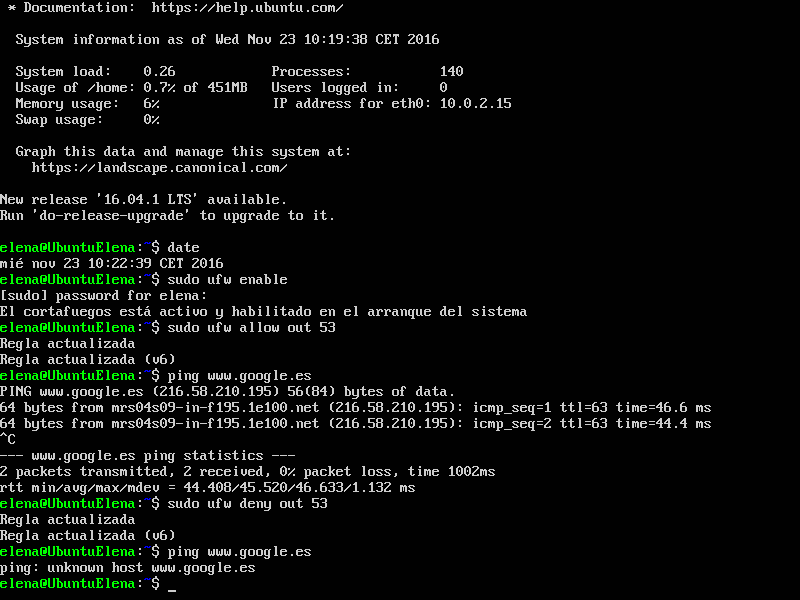
\includegraphics[width=15cm]{./img/ejercicio3a.png} 	
	\caption{Ubuntu Server, abrir y cerrar un puerto con ufw.} \label{fig:ejercicio3a}
\end{figure}

\subsection{b) ¿Con qué comando puede abrir/cerrar un puerto usando firewall-cmd en CentOS? Muestre un ejemplo de cómo lo ha hecho }
Tal y como se indica en el man de CentOS:
\begin{enumerate}
	\item Para abrir un puerto se usa el comando: \texttt{firewall-cmd --add-port=<port>/<protocol>}.
	\item Para cerrar un puerto se usa el comando: \texttt{firewall-cmd --remove-port=<port>/<protocol>}. 
\end{enumerate}

Por ejemplo abro y cierro el puerto 53, como se muestra en la figura \ref{fig:ejercicio3b}.
\begin{figure}[H] 
	\centering
	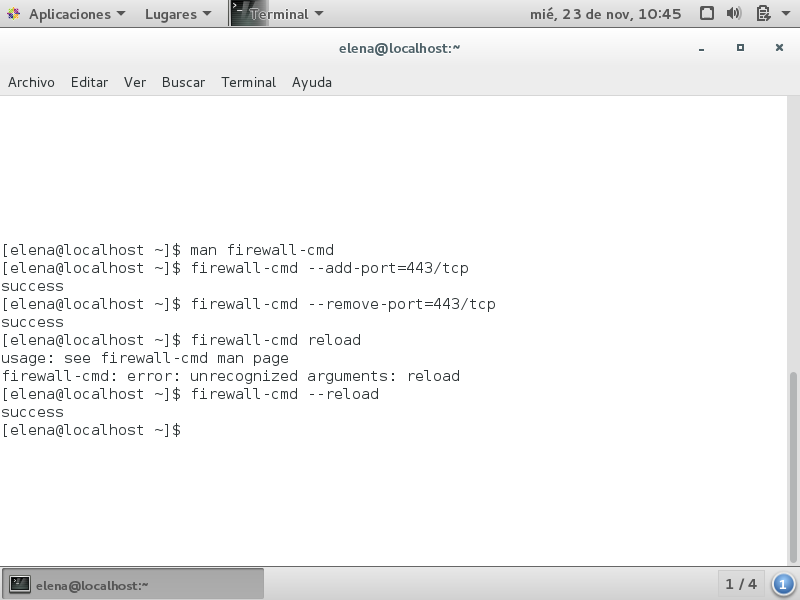
\includegraphics[width=15cm]{./img/ejercicio3b.png} 	
	\caption{CentOS, abrir y cerrar un puerto con firewall-cmd.} \label{fig:ejercicio3b}
\end{figure}

Comprobamos que aparece en el cortafuegos de CentOS el puerto 443, como se ve en la figura \ref{fig:ejercicio3b443a}, que previamente hemos habilitado. Después de cerrar el puerto 443 el cortafuegos ya no lo detecta como se muestra en la figura \ref{fig:ejercicio3b443b}.
\begin{figure}[H] 
	\centering
	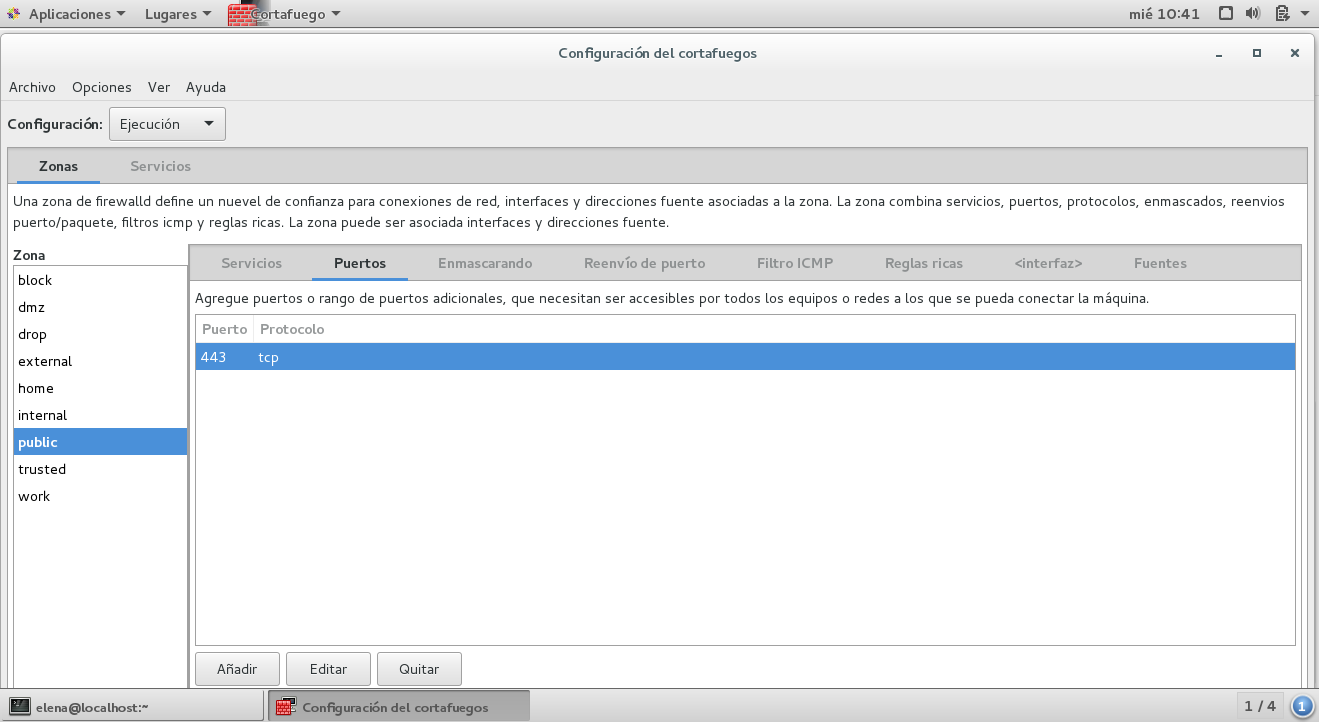
\includegraphics[width=15cm]{./img/ejercicio3b443a.png} 	
	\caption{CentOS, despues de abrir el puerto 443 con firewall-cmd.} \label{fig:ejercicio3b443a}
\end{figure}
\begin{figure}[H] 
	\centering
	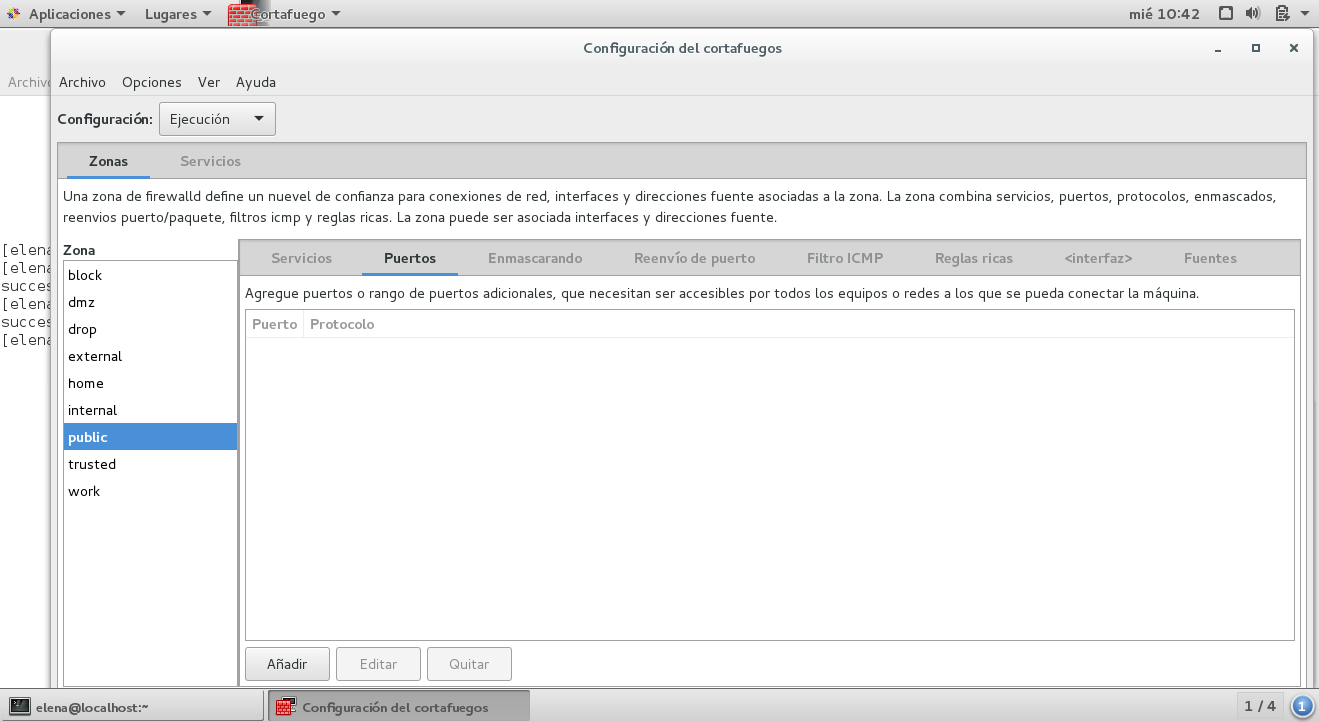
\includegraphics[width=15cm]{./img/ejercicio3b443b.png} 	
	\caption{CentOS, despues de cerrar el puerto 443 con firewall-cmd.} \label{fig:ejercicio3b443b}
\end{figure}


\subsection{c) Utilice el comando nmap para ver que, efectivamente, los puertos están accesibles}
Para utilizar el comando nmap voy a probarlo sobre el puerto 22 (puerto de shh) desde CentOS hacia Ubuntu Server. Para ello primero en Ubuntu Server habilito el cortafuegos y el puerto 22 como se muestra en la figura \ref{fig:ejercicio3c1}. Desde CentOS compruebo que efectivamente tengo acceso con ssh al servidor de Ubuntu (figura \ref{fig:ejercicio3c2}).
Utilizando el comando nmap desde CentOS podemos verificar que el puerto está abierto, aparece ``open'' (figura \ref{fig:ejercicio3c3}).


\begin{figure}[H] 
	\centering
	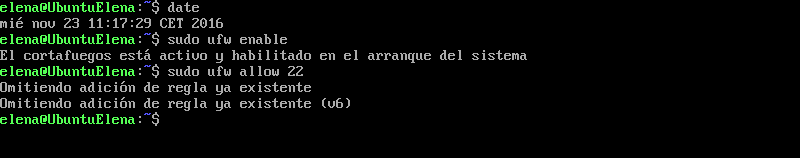
\includegraphics[width=15cm]{./img/ejercicio3c1.png} 	
	\caption{Ubuntu, abrir el puerto 22 con ufw.} \label{fig:ejercicio3c1}
\end{figure}

\begin{figure}[H] 
	\centering
	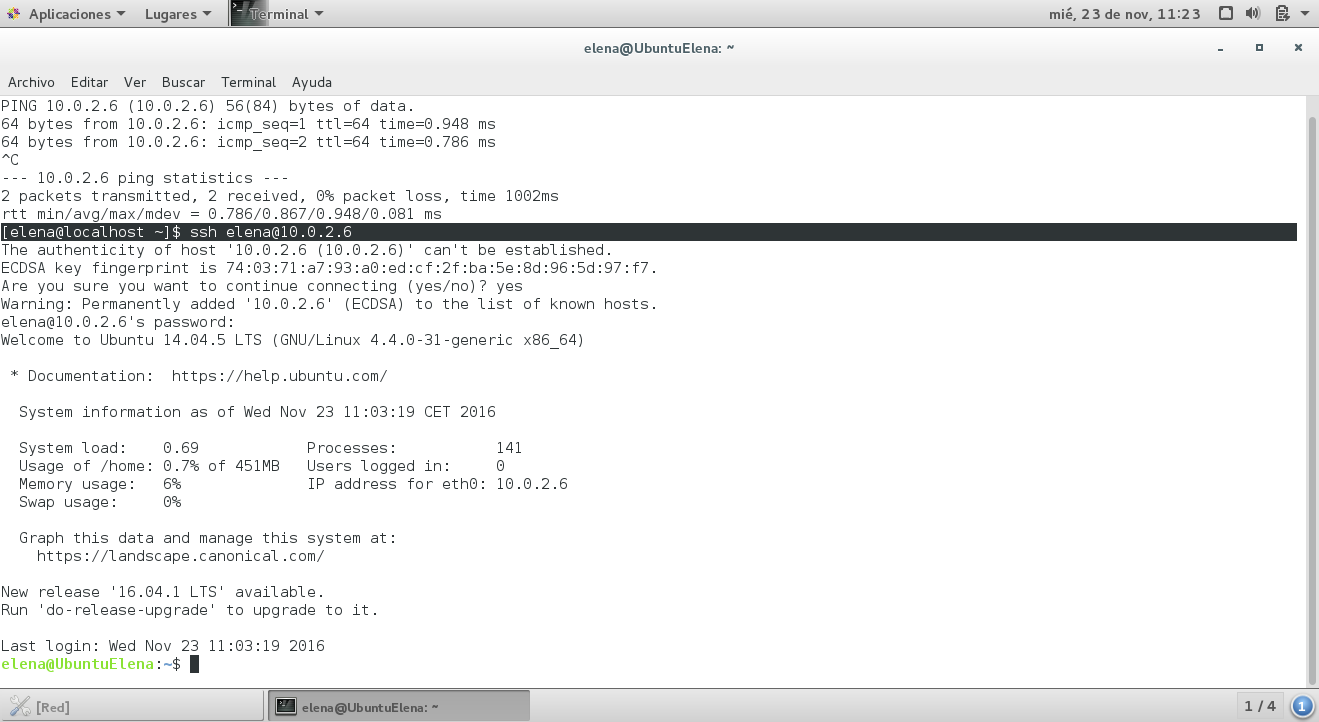
\includegraphics[width=15cm]{./img/ejercicio3c2.png} 	
	\caption{CentOS, conexión con ssh a Ubuntu Server.} \label{fig:ejercicio3c2}
\end{figure}

\begin{figure}[H] 
	\centering
	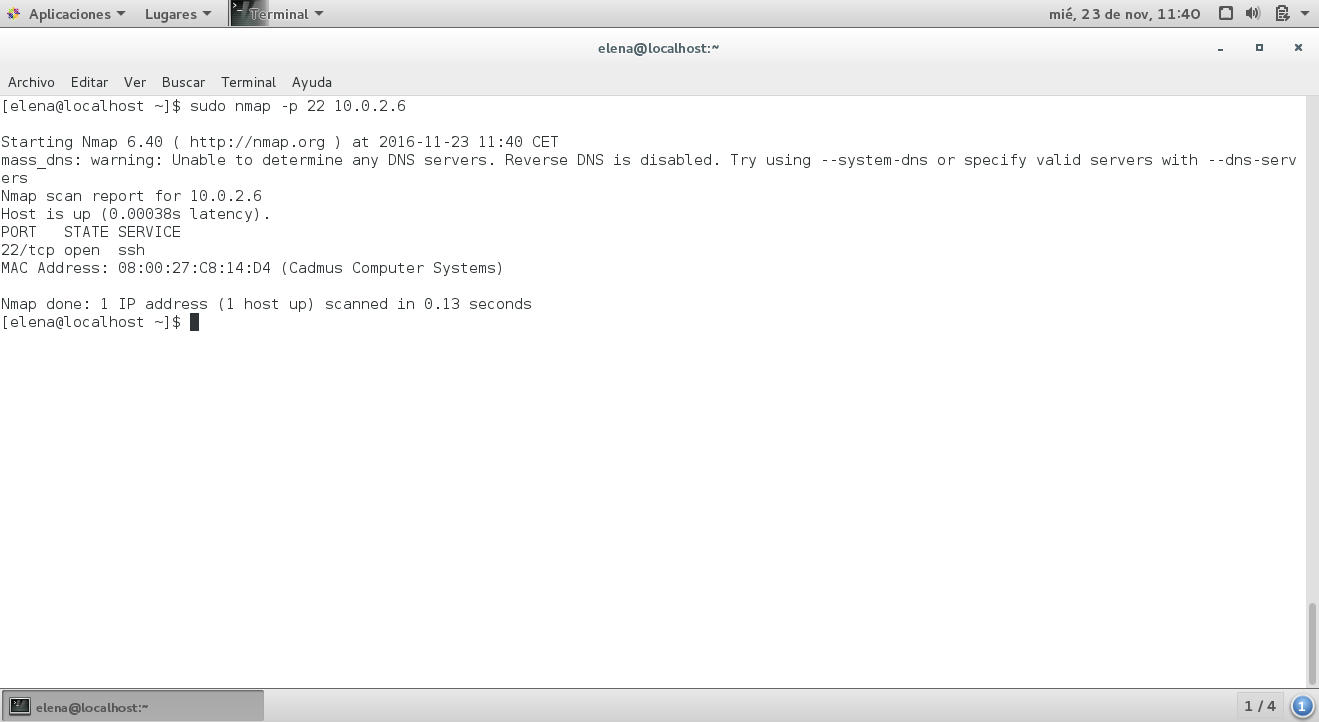
\includegraphics[width=15cm]{./img/ejercicio3c3.png} 	
	\caption{CentOS, nmap hacia Ubuntu Server.} \label{fig:ejercicio3c3}
\end{figure}

Ahora vamos a proceder a cerrar el puerto 22 en Ubuntu (figura \ref{fig:ejercicio3c4}) y comprobamos desde CentOS con nmap que está cerrado, aparece ``filtered'' (figura \ref{fig:ejercicio3c5}).

\begin{figure}[H] 
	\centering
	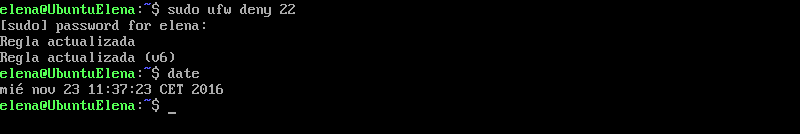
\includegraphics[width=15cm]{./img/ejercicio3c4.png} 	
	\caption{Ubuntu, cerrar el puerto 22 con ufw.} \label{fig:ejercicio3c4}
\end{figure}

\begin{figure}[H] 
	\centering
	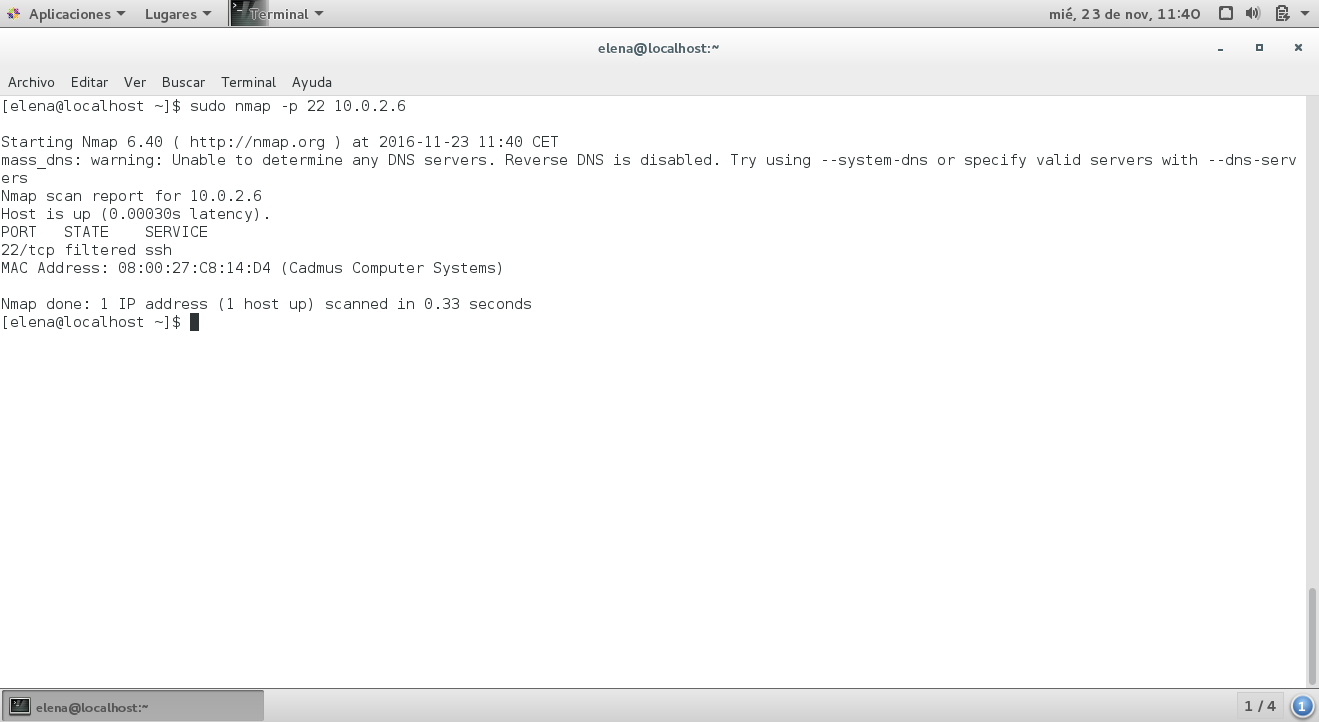
\includegraphics[width=15cm]{./img/ejercicio3c5.png} 	
	\caption{CentOS, nmap hacia Ubuntu Server.} \label{fig:ejercicio3c5}
\end{figure}


%----------------------------------------------------------------------------------------
%	Cuestión 4
%----------------------------------------------------------------------------------------

\section{Cuestión 4: ¿Qué diferencia hay entre telnet y ssh?}
Tal y como hemos visto en la asignatura de fundamentos de redes, la principal diferencia entre \texttt{SSH} y \texttt{Telnet} es que,   aunque ambos sirven para acceder a máquinas remotas a través de una red, \texttt{SSH} lo hace cifrando los datos, de manera que ofrece  mayor seguridad que \texttt{Telnet}.


%----------------------------------------------------------------------------------------
%	Cuestión 5
%----------------------------------------------------------------------------------------

\section{Cuestión 5:}

\subsection{a) ¿Para qué sirve la opción -X? }
Tal y como se dice en el man de ssh \cite{sshX}, la opción -X sirve para habilitar el reenvío X11, el cuál debe ser activado con precaución ya que permite la posibilidad de acceder a la pantalla local o monitorizar las pulsaciones.

\subsection{b) Ejecute remotamente, es decir, desde la máquina anfitriona (si tiene Linux) o desde la otra máquina virtual, el comando gedit en una sesión abierta con ssh. ¿Qué ocurre?}

Como se puede apreciar en la figura \ref{fig:ejercicio5b}, no es posible ejecutar gedit ya que por defecto ssh no tiene habilitado X11. Para poder ejecutar gedit (figura \ref{fig:ejercicio5b3}) tenemos que utilizar la opción -X de ssh (figura \ref{fig:ejercicio5b2}), que está explicada en el ejercicio anterior. Para comprobar que ha funcionado correctamente accedemos al archivo creado en Ubuntu Server con gedit desde CentOS (figura \ref{fig:ejercicio5b4}).

\begin{figure}[H] 
	\centering
	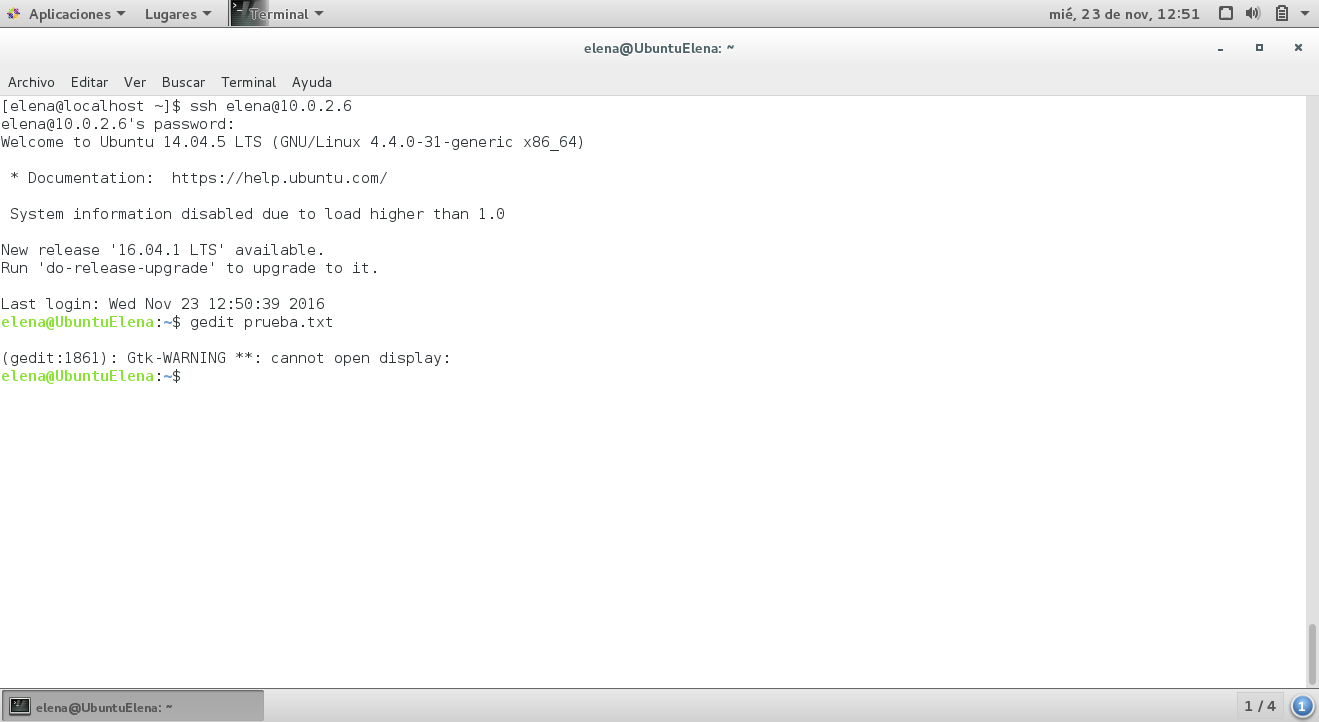
\includegraphics[width=15cm]{./img/ejercicio5b.png} 	
	\caption{CentOS, gedit ejecutado remotamente hacia Ubuntu, con error.} \label{fig:ejercicio5b}
\end{figure}

\begin{figure}[H] 
	\centering
	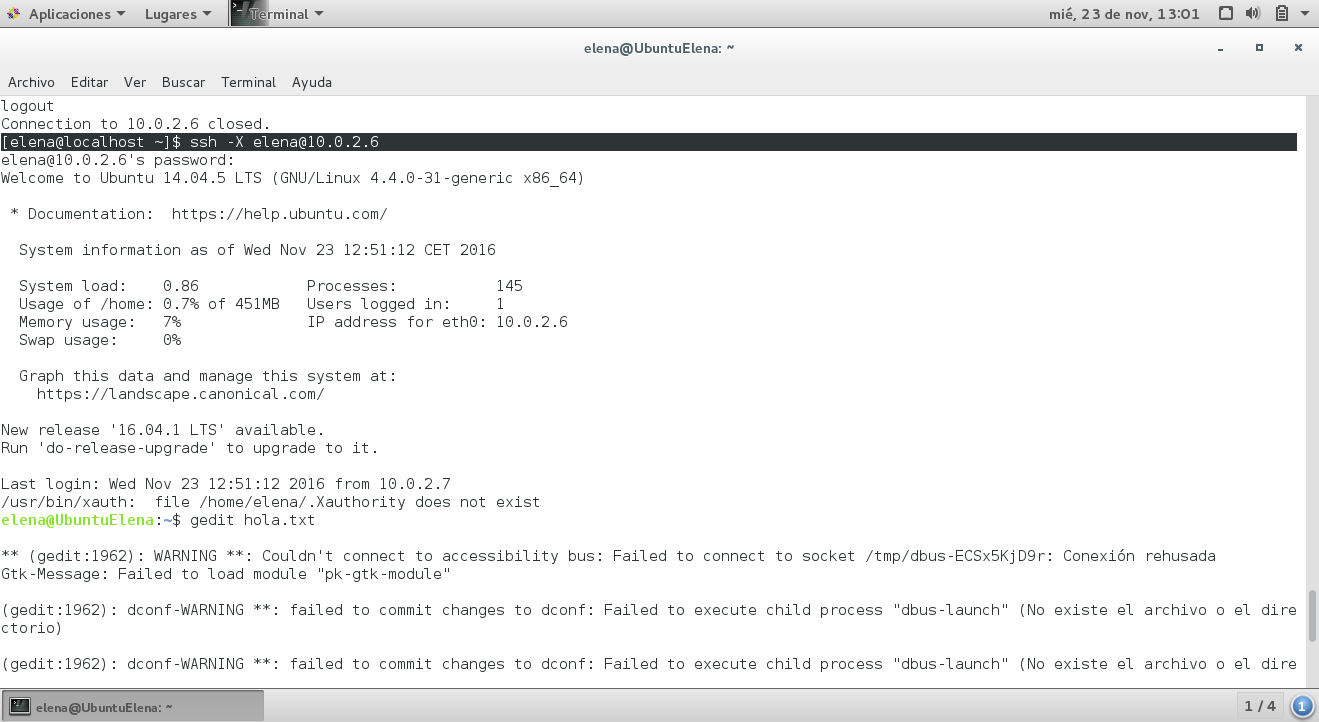
\includegraphics[width=15cm]{./img/ejercicio5b2.png} 	
	\caption{CentOS, ssh con opción X11 habilitado.} \label{fig:ejercicio5b2}
\end{figure}

\begin{figure}[H] 
	\centering
	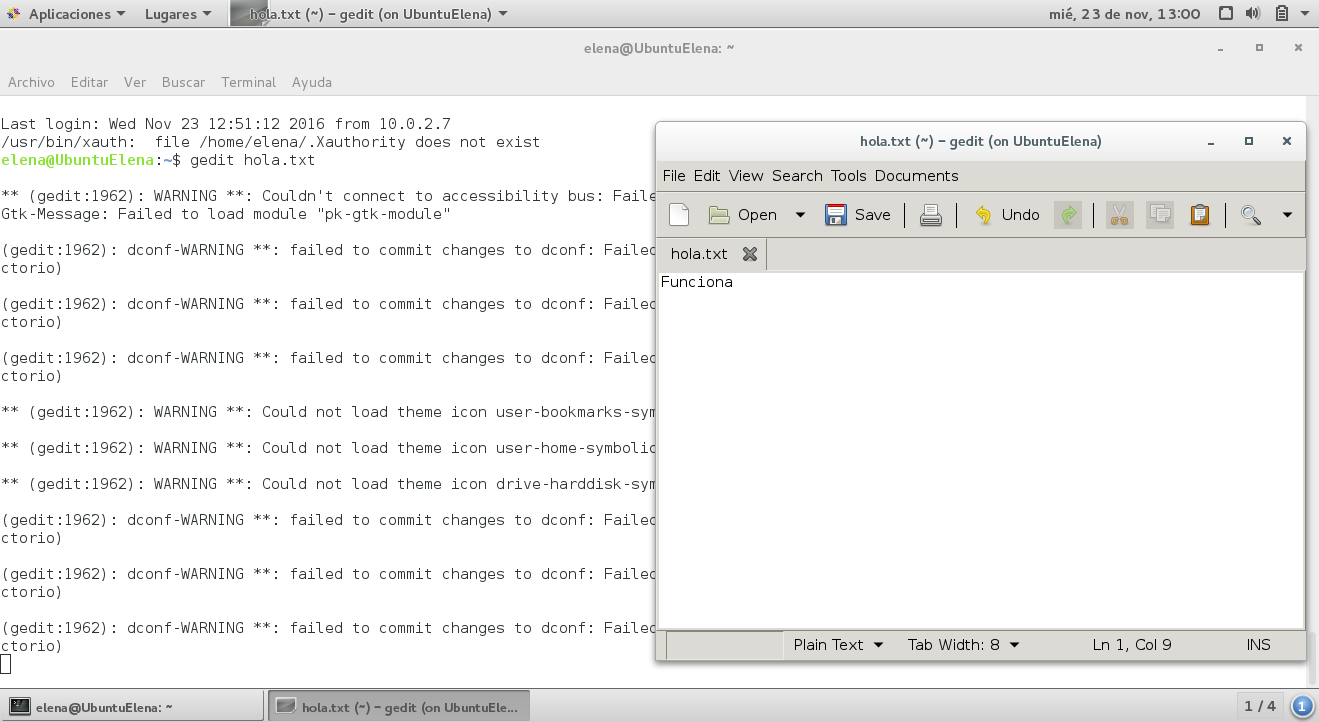
\includegraphics[width=15cm]{./img/ejercicio5b3.png} 	
	\caption{CentOS, gedit ejecutado remotamente hacia Ubuntu.} \label{fig:ejercicio5b3}
\end{figure}

\begin{figure}[H] 
	\centering
	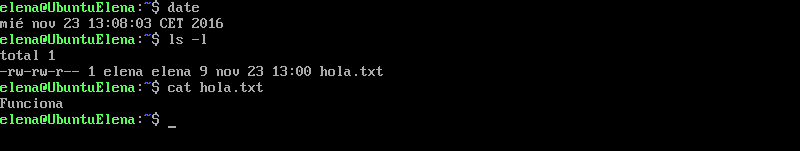
\includegraphics[width=15cm]{./img/ejercicio5b4.png} 	
	\caption{Ubuntu Server, comprobación de la creación del archivo de forma remota.} \label{fig:ejercicio5b4}
\end{figure}


%----------------------------------------------------------------------------------------
%	Cuestión 6
%----------------------------------------------------------------------------------------

\section{Cuestión 6: muestre la secuencia de comandos y las modificaciones a los archivos correspondientes para permitir acceder a la consola remota sin introducir la contraseña. Pruebe que funciona. (Pistas: ssh-keygen, ssh-copy- id).}
Para poder acceder a la consola remota sin introducir la contraseña es necesario realizar los siguientes pasos, tal y como se indica en la ayuda de Ubuntu \cite{sshPass}.\\

Primero generamos la clave pública y privada con \texttt{ssh-keygen -t rsa} (figura \ref{fig:ejercicio6-1}).
Una vez generada copiamos la clave en la máquina remota con \texttt{ssh-­copy-­id username@remotehost} (figura \ref{fig:ejercicio6-2}).
Ahora tenemos que editar el fichero de configuración de ssh, con \texttt{sudo nano /etc/ssh/sshd\_config} y cambiamos la línea ``StrictModes yes'' por ``StrictModes no'' (figura \ref{fig:ejercicio6-3}). Finalmente reiniciamos el servidor ssh con \texttt{/etc/init.d/ssh restart}. En la figura \ref{fig:ejercicio6-4} compruebo que puedo hacer la conexión sin necesidad de introducir contraseña.


\begin{figure}[H] 
	\centering
	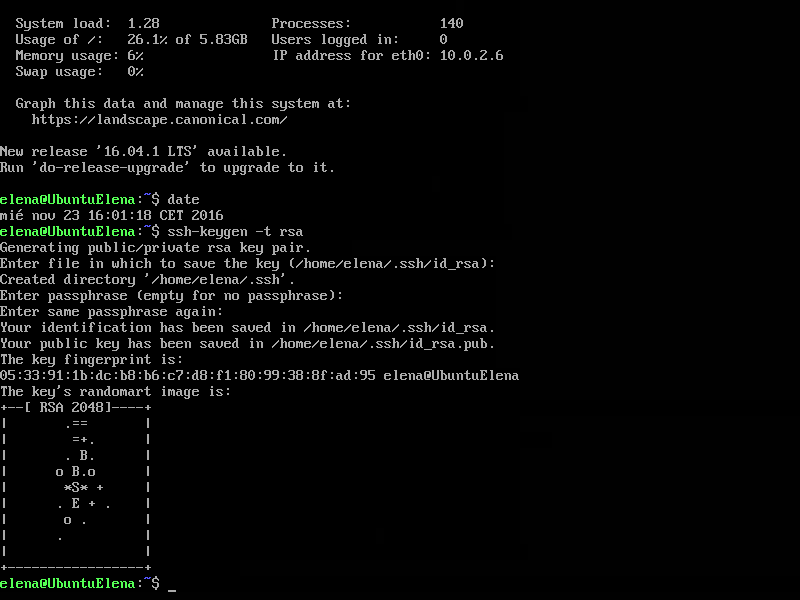
\includegraphics[width=15cm]{./img/ejercicio6-1.png} 	
	\caption{Ubuntu Server, generar clave pública y privada ssh.} \label{fig:ejercicio6-1}
\end{figure}

\begin{figure}[H] 
	\centering
	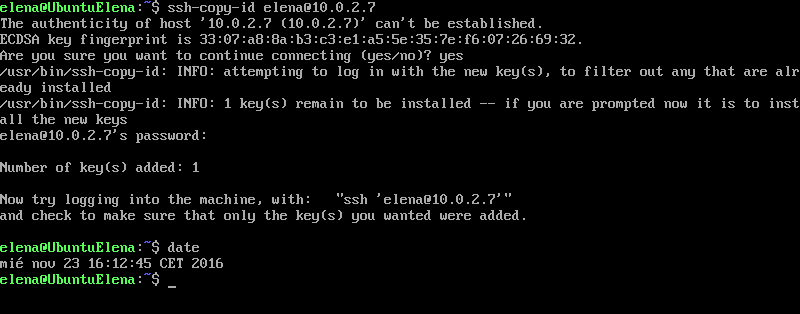
\includegraphics[width=15cm]{./img/ejercicio6-2.png} 	
	\caption{Ubuntu Server, copiar clave pública ssh.} \label{fig:ejercicio6-2}
\end{figure}

\begin{figure}[H] 
	\centering
	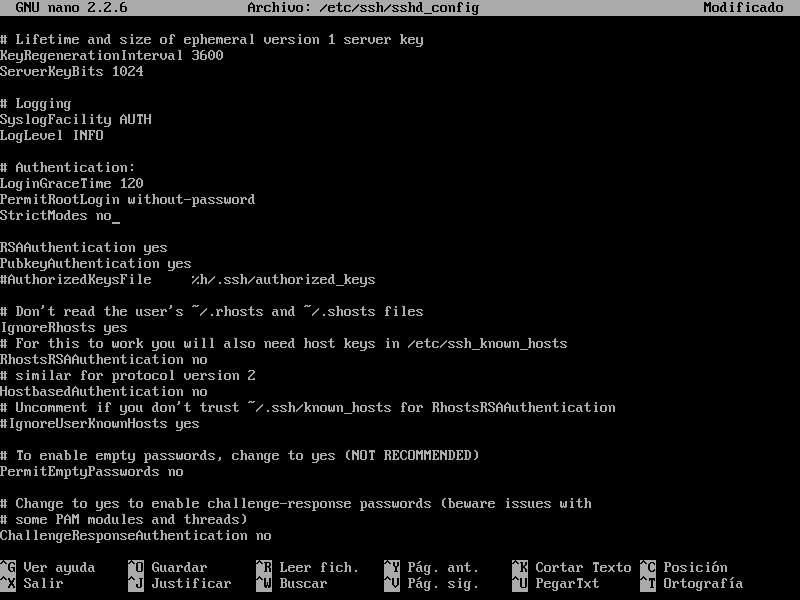
\includegraphics[width=15cm]{./img/ejercicio6-3.png} 	
	\caption{Ubuntu Server, configuración ssh.} \label{fig:ejercicio6-3}
\end{figure}

\begin{figure}[H] 
	\centering
	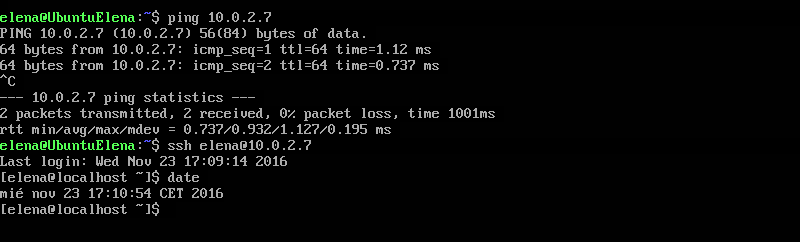
\includegraphics[width=15cm]{./img/ejercicio6-4.png} 	
	\caption{Ubuntu Server, conexión sin contraseña a CentOS.} \label{fig:ejercicio6-4}
\end{figure}



%----------------------------------------------------------------------------------------
%	Cuestión 7
%----------------------------------------------------------------------------------------
\section{Cuestión 7: ¿Qué archivo es el que contiene la configuración del servicio ssh? ¿Qué parámetro hay que modificar para evitar que el usuario root acceda? Cambie el puerto por defecto y compruebe que puede acceder.}
 Tal y como se dice en la ayuda de Ubuntu \cite{sshPass}, el archivo que contiene la configuración del servicio ssh es \texttt{/etc/ssh/sshd\_config}.
 Para evitar acceder al usuario root hay que modificar en el archivo de configuración buscando la línea \texttt{\# PermitRootLogin no} y descomentándola, o creándola si no existe, tal y como se indica en \cite{sshConfig} (figura \ref{fig:ejercicio7-1}). Para que los cambios funcionen se debe reiniciar el servicio del SSH con \texttt{systemctl restart sshd}. Como se puede ver en la figura \ref{fig:ejercicio7-2} ahora no permite acceso al root.\\

Para cambiar el puerto lo que se debe hacer es buscar la línea \texttt{Port 22} dentro del archivo de configuración \texttt{/etc/ssh/sshd\_config} y \texttt{/etc/ssh/ssh\_config}y cambiar el puerto 22 por un puerto libre, yo lo he cambiado tanto en CentOS (figura \ref{fig:ejercicio7-3}, figura \ref{fig:ejercicio7-7}) como en Ubuntu Server (figura \ref{fig:ejercicio7-4}, figura \ref{fig:ejercicio7-6}) por el puerto 2222. Como se puede observar en la figura \ref{fig:ejercicio7-5} puedo seguir accediendo sin problema después de cambiar el puerto.
 
 
\begin{figure}[H] 
	\centering
	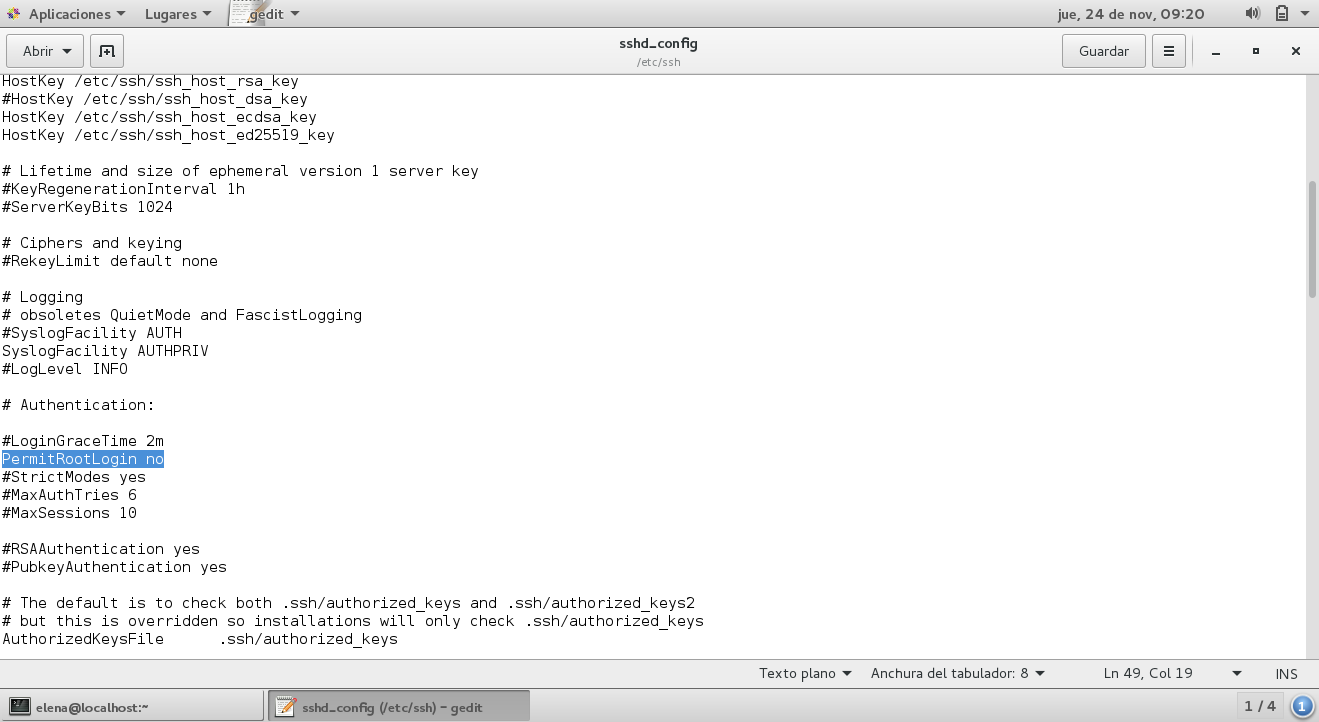
\includegraphics[width=15cm]{./img/ejercicio7-1.png} 	
	\caption{CentOS, configuracion ssh: evitar acceso a root.} \label{fig:ejercicio7-1}
\end{figure}

\begin{figure}[H] 
	\centering
	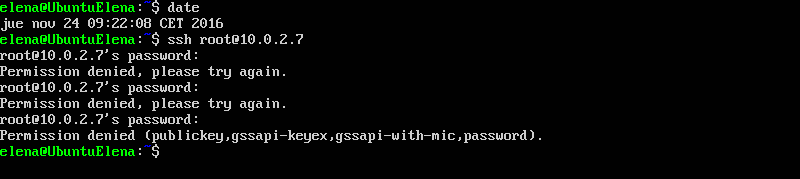
\includegraphics[width=15cm]{./img/ejercicio7-2.png} 	
	\caption{Ubuntu Server, configuracion ssh: evitar acceso a root.} \label{fig:ejercicio7-2}
\end{figure}

\begin{figure}[H] 
	\centering
	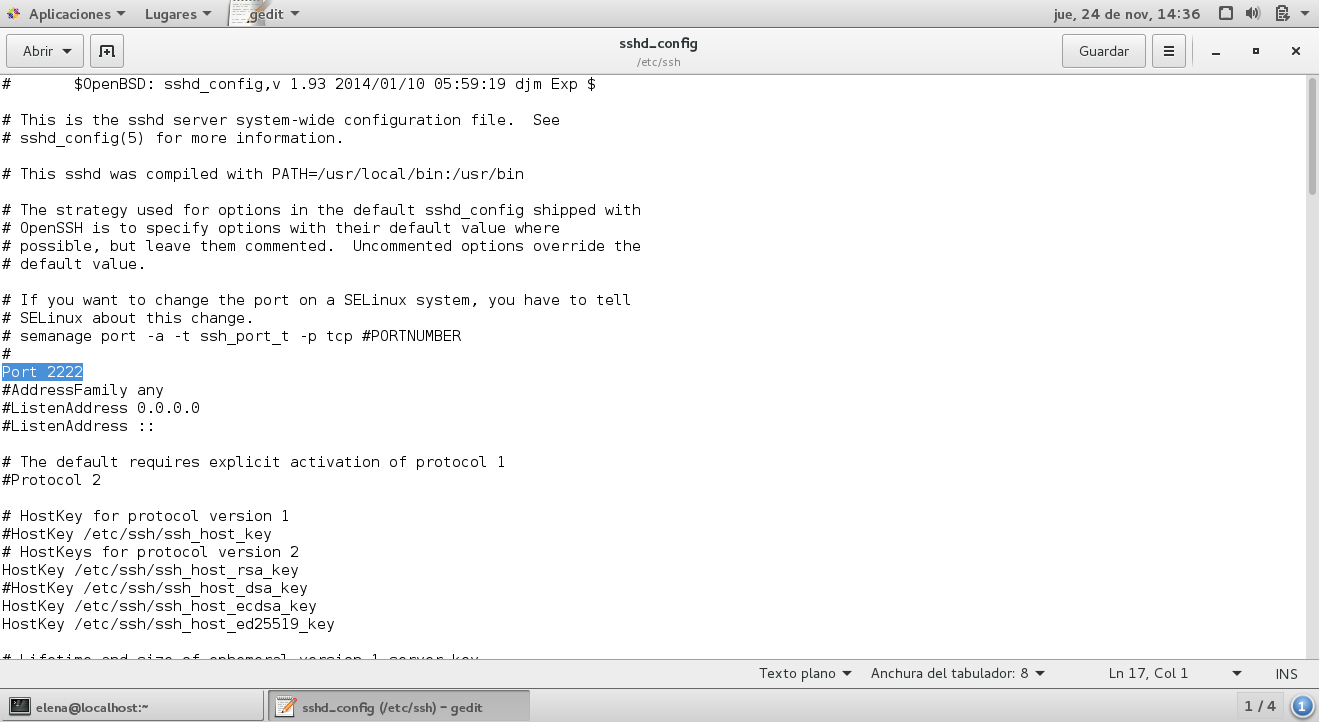
\includegraphics[width=15cm]{./img/ejercicio7-3.png} 	
	\caption{CentOS, configuracion ssh: cambio de puerto.} \label{fig:ejercicio7-3}
\end{figure}

\begin{figure}[H] 
	\centering
	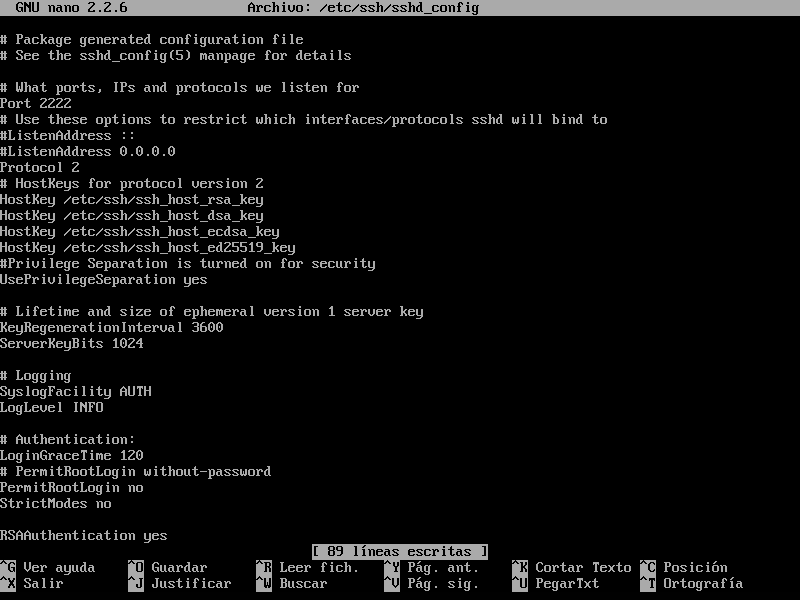
\includegraphics[width=15cm]{./img/ejercicio7-4.png} 	
	\caption{Ubuntu Server, configuracion ssh: cambio de puerto.} \label{fig:ejercicio7-4}
\end{figure}

\begin{figure}[H] 
	\centering
	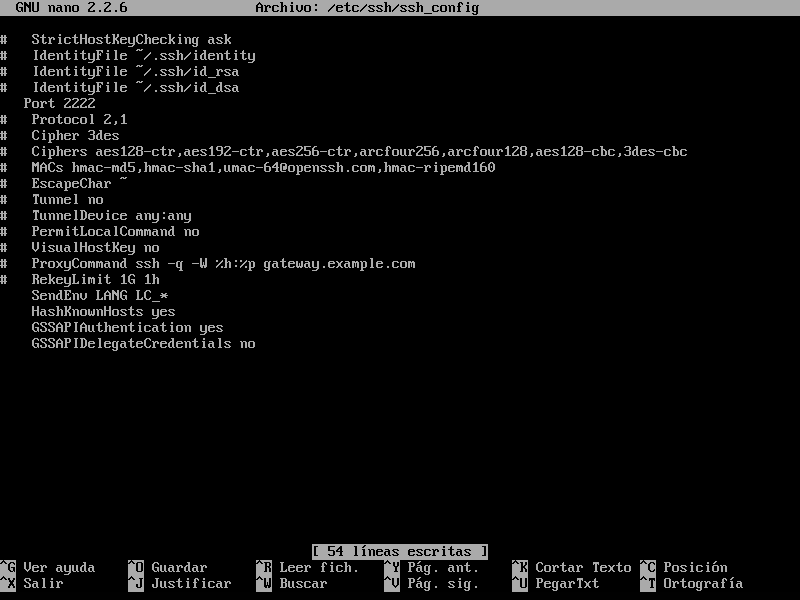
\includegraphics[width=15cm]{./img/ejercicio7-6.png} 	
	\caption{Ubuntu Server, configuracion ssh: cambio de puerto.} \label{fig:ejercicio7-6}
\end{figure}

\begin{figure}[H] 
	\centering
	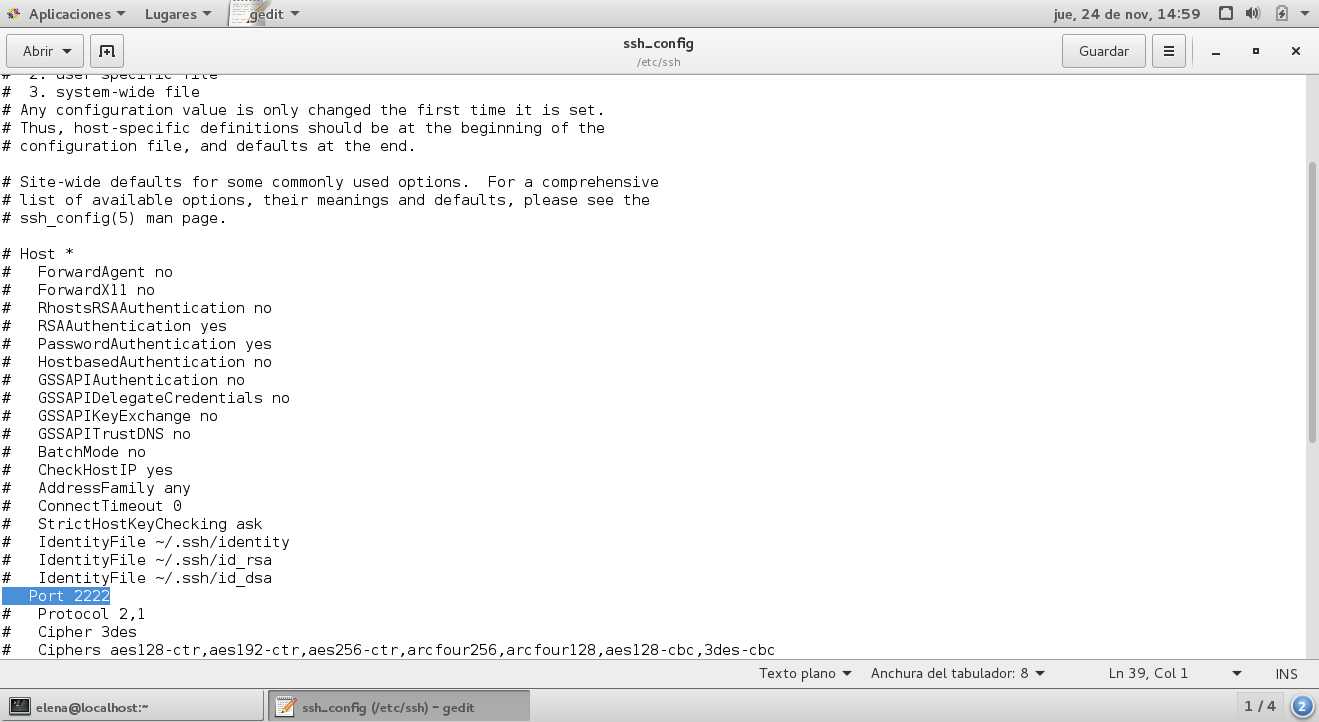
\includegraphics[width=15cm]{./img/ejercicio7-7.png} 	
	\caption{CentOS, configuracion ssh: cambio de puerto.} \label{fig:ejercicio7-7}
\end{figure}

\begin{figure}[H] 
	\centering
	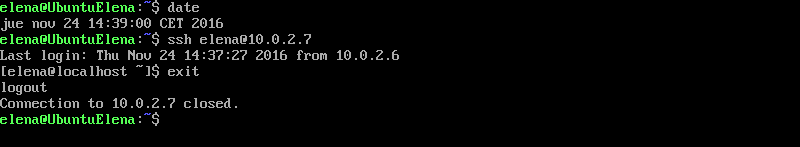
\includegraphics[width=15cm]{./img/ejercicio7-5.png} 	
	\caption{Ubuntu Server, conexión mediante ssh con puerto cambiado.} \label{fig:ejercicio7-5}
\end{figure}

%----------------------------------------------------------------------------------------
%  Cuestión 8
%----------------------------------------------------------------------------------------

\section{Cuestión 8: Indique si es necesario reiniciar el servicio ¿Cómo se reinicia un servicio en Ubuntu? ¿y en CentOS? Muestre la secuencia de comandos para hacerlo.}
Siempre que se haga algún cambio en el archivo de configuración del ssh se debe reiniciar el servicio. Hay distintas formas para reiniciar los servicios, una de ellas es la siguiente:\\

En CentOS con el comando \texttt{service sshd restart} (figura \ref{fig:ejercicio8-2}).\\
En Ubuntu server con el comando \texttt{sudo restart ssh} (figura \ref{fig:ejercicio8-1}).


\begin{figure}[H] 
	\centering
	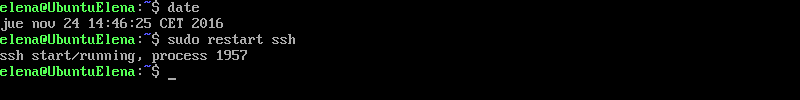
\includegraphics[width=15cm]{./img/ejercicio8-1.png} 	
	\caption{Ubuntu Server, reinicio del servicio ssh.} \label{fig:ejercicio8-1}
\end{figure}

\begin{figure}[H] 
	\centering
	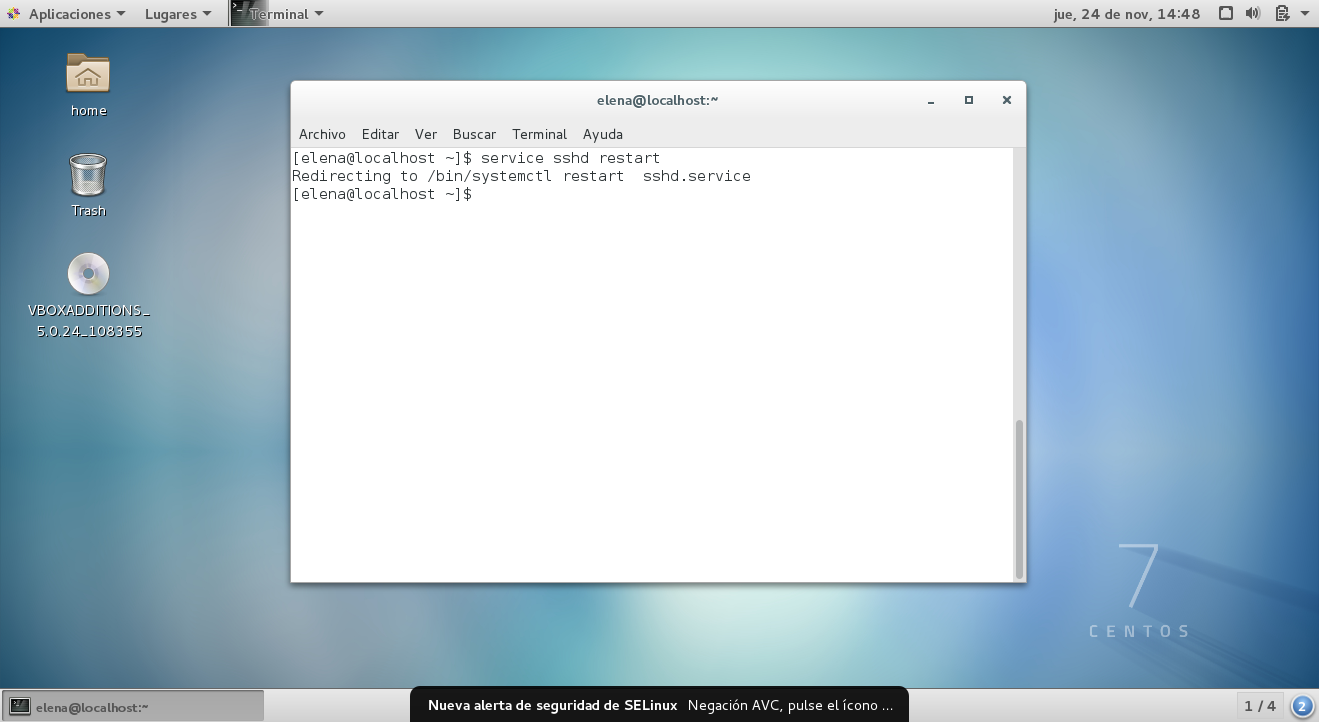
\includegraphics[width=15cm]{./img/ejercicio8-2.png} 	
	\caption{CentOS, reinicio del servicio ssh.} \label{fig:ejercicio8-2}
\end{figure}

%----------------------------------------------------------------------------------------
%  Cuestión opcional 1
%----------------------------------------------------------------------------------------

\section{Cuestión opcional 1 : Instale y pruebe terminator y/o tmux. Con screen, pruebe su funcionamiento dejando sesiones ssh abiertas en el servidor y recuperándolas posteriormente.}
Instalo en CentOS screen y tmux, con \texttt{yum install screen} con \texttt{yum install tmux} respectivamente.

Tmux sirve para tener varias terminales abiertas como se muestra en la figura \ref{fig:opcional1a}. Tmux funciona con varios atajos de teclado, para crear una nueva ventana simplemente debemos poner tmux, y para que se vean varias juntas podemos hacerlo horizontalmente con \texttt{(Ctrl-b) + “} o verticalmente con  \texttt{(Ctrl-b) + \%} como se indica en \cite{tmux}.


\begin{figure}[H] 
	\centering
	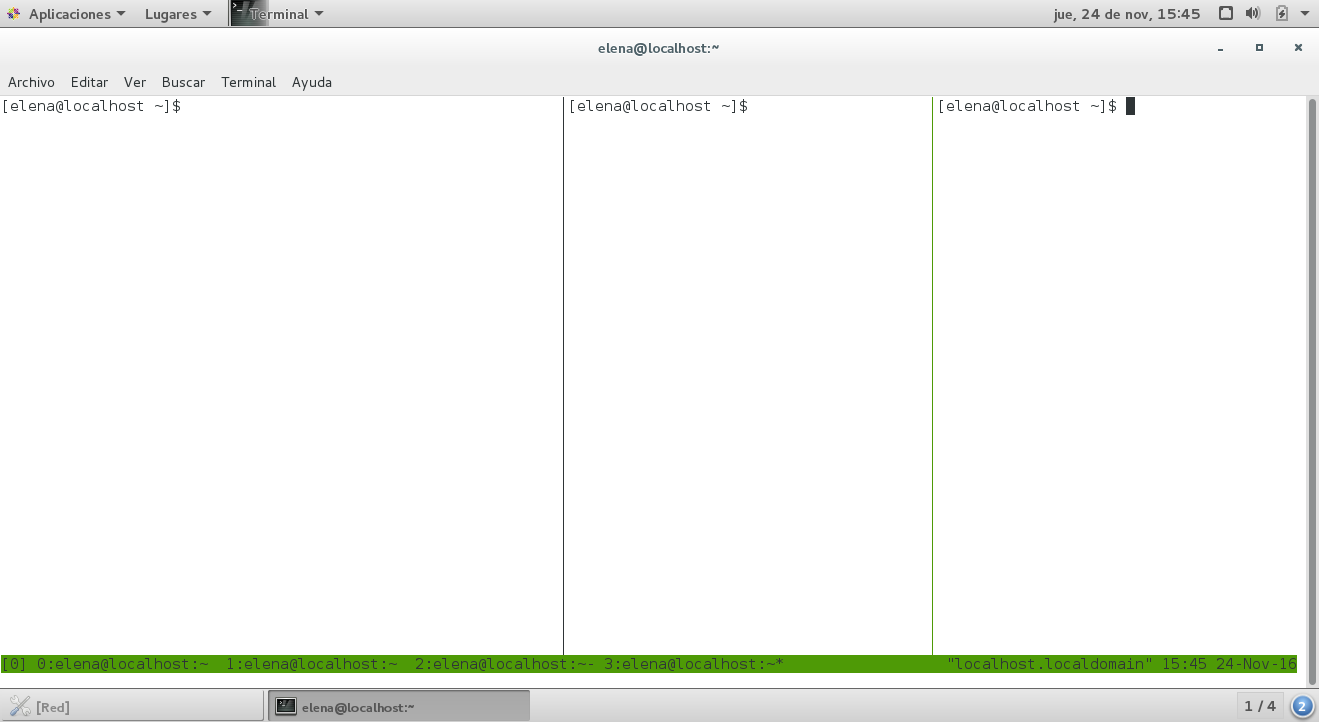
\includegraphics[width=15cm]{./img/opcional1a.png} 	
	\caption{CentOS, ejemplo de tmux.} \label{fig:opcional1a}
\end{figure}

Para comprobar el funcionamiento de screen \cite{screen}, primero me conecto mediante ssh a Ubuntu Server (figura \ref{fig:opcional1b}) y lanzo una segunda terminal en el ssh con \texttt{screen bash}, para dejar la terminal de screen abierta ejecutamos \texttt{CTRL+A} y a continuación \texttt{CTRL+D} y ya podemos cerrar la terminal ssh original con \texttt{exit} (figura \ref{fig:opcional1c}). Para recuperar la sesión activa posteriormente se hace mediante el comando \texttt{screen -r}, para comprobar el correcto funcionamiento yo lo que he hecho ha sido dejar el man de gedit abierto en la terminal abierta con screen, y al volver a la sesión abierta con \texttt{screen -r} seguía estando el man abierto tal y como lo dejé (figura \ref{fig:opcional1d}). 

\begin{figure}[H] 
	\centering
	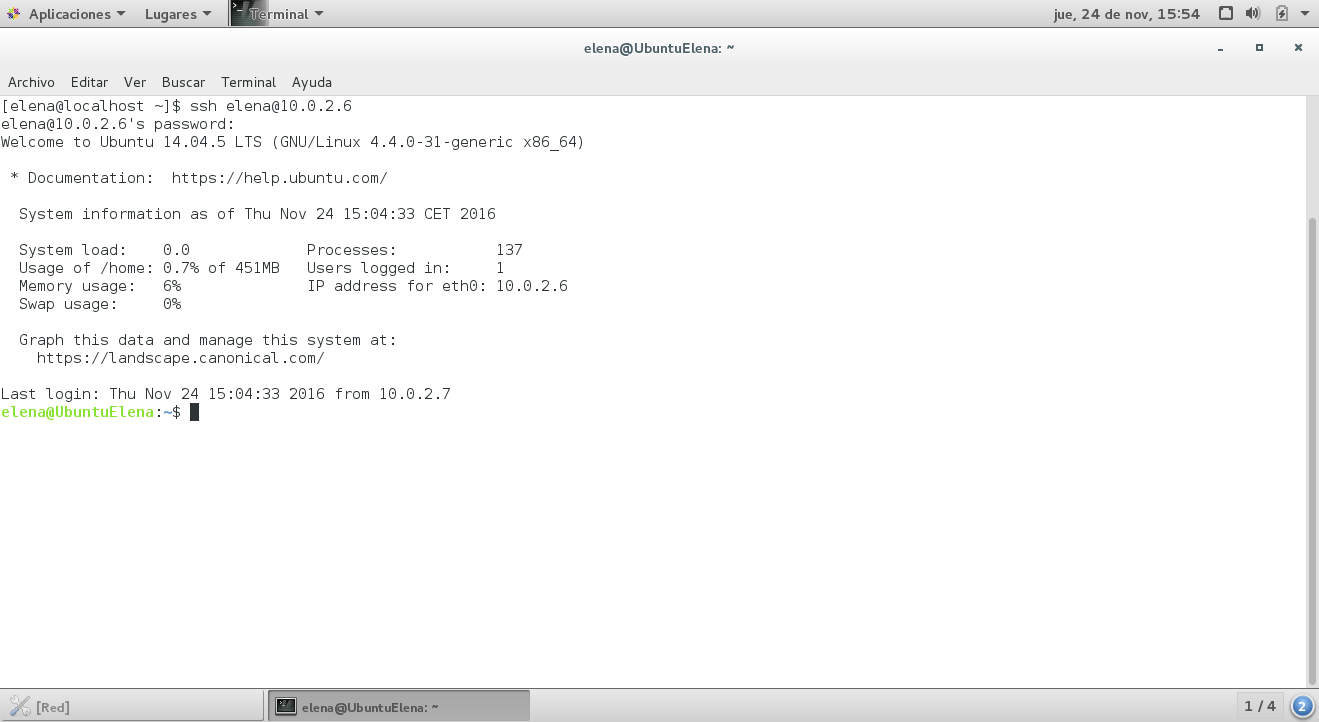
\includegraphics[width=15cm]{./img/opcional1b.png} 	
	\caption{CentOS, ejemplo de screen.} \label{fig:opcional1b}
\end{figure}

\begin{figure}[H] 
	\centering
	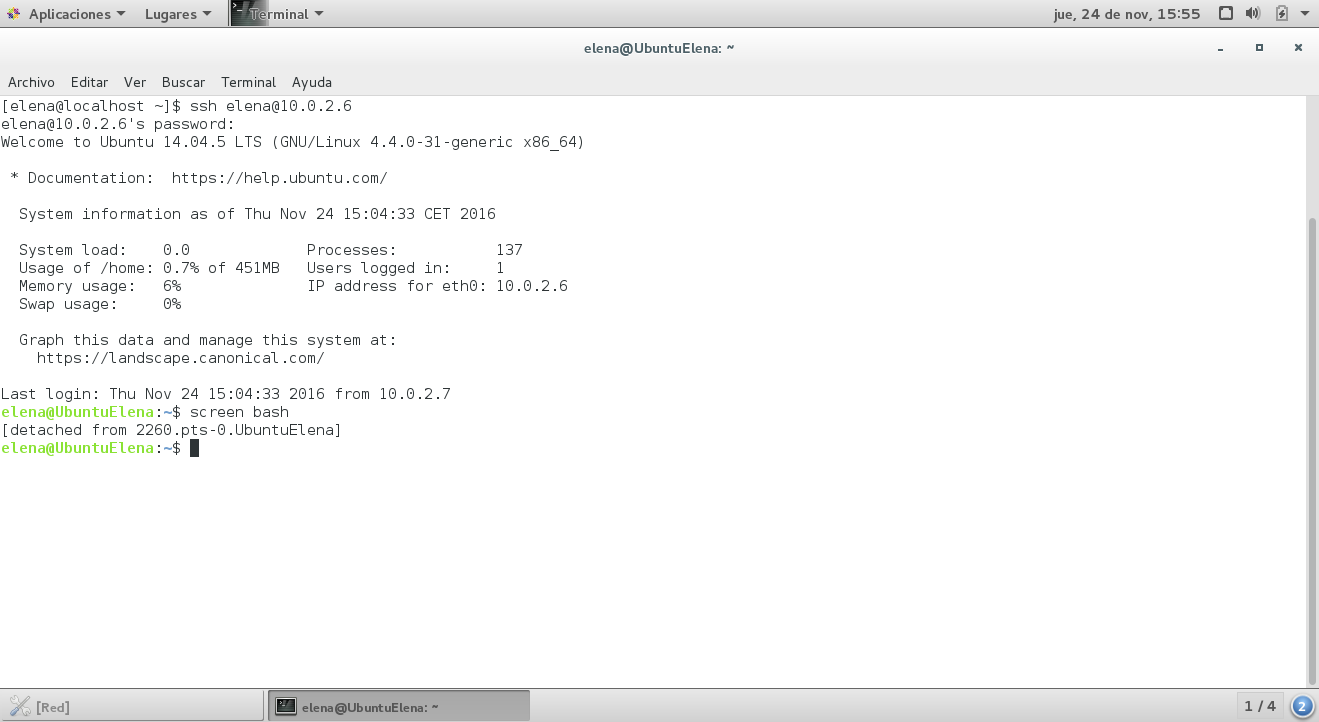
\includegraphics[width=15cm]{./img/opcional1c.png} 	
	\caption{CentOS, ejemplo de screen.} \label{fig:opcional1c}
\end{figure}

\begin{figure}[H] 
	\centering
	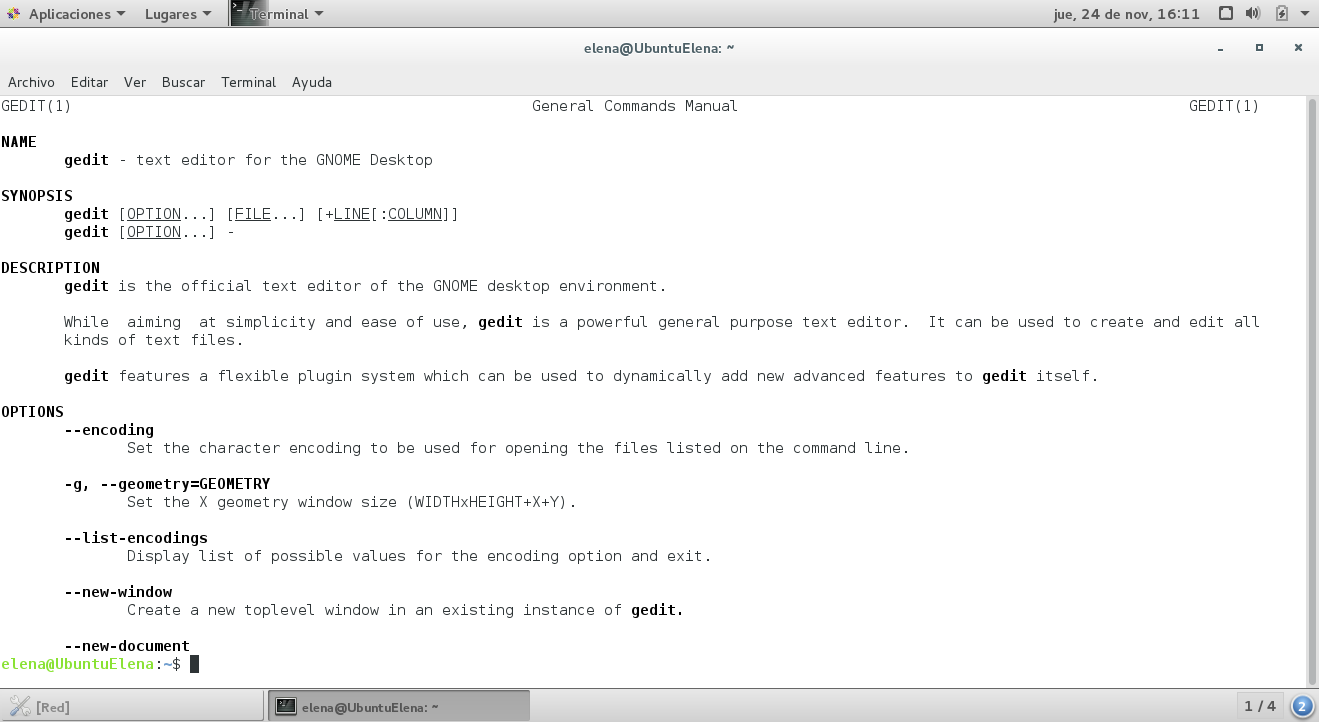
\includegraphics[width=15cm]{./img/opcional1d.png} 	
	\caption{CentOS, ejemplo de screen.} \label{fig:opcional1d}
\end{figure}


%----------------------------------------------------------------------------------------
%  Cuestión opcional 2
%----------------------------------------------------------------------------------------

\section{Cuestión opcional 2 : Instale el servicio y pruebe su funcionamiento.}
Se instala con el comando \texttt{yum install fail2ban} (figura \ref{fig:opcional2b}), pero previamente debemos instalar el repositorio EPEL con \texttt{yum install epel-release} (figura \ref{fig:opcional2a}) que contiene paquetes adicionales para CentOS, tal y como se indica en \cite{fail2ban}. La configuración se encuentra en el archivo \texttt{/etc/fail2ban/jail.conf}. El parámetro ignoreip sirve para agregar IPs que no queremos que sean bloqueadas por error a la lista blanca, como por ejemplo nuestra propia IP para que nunca perdamos el acceso a nuestro servidor. Se debe reiniciar el servicio con \texttt{sudo service fail2ban restart}.

Creamos un nuevo archivo con \texttt{nano /etc/fail2ban/jail.d/sshd.local}, e introducimos las siguientes líneas:\\
$[$sshd$]$\\
enabled = true\\
port = ssh\\
\#action = firewallcmd-ipset\\
logpath = \%(sshd\_log)s\\
maxretry = 5\\
bantime = 86400\\

\begin{figure}[H] 
	\centering
	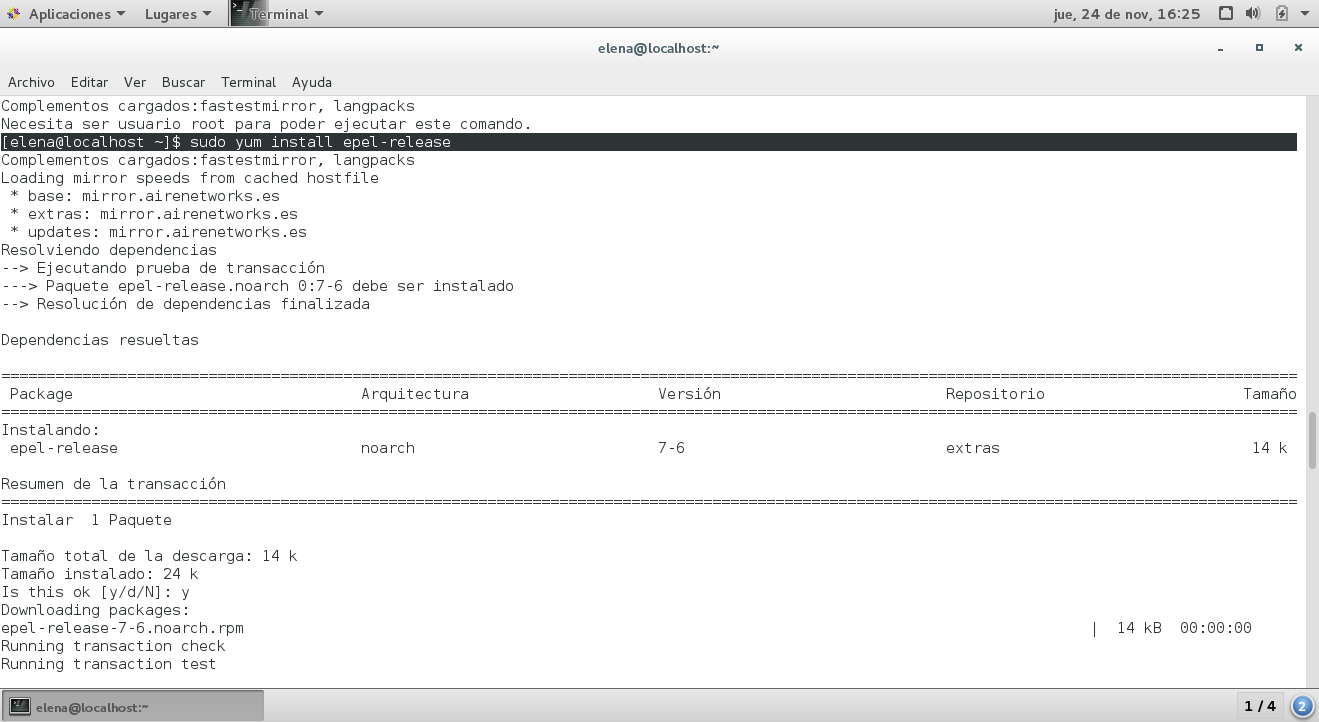
\includegraphics[width=15cm]{./img/opcional2a.png} 	
	\caption{CentOS, instalar epel.} \label{fig:opcional2a}
\end{figure}

\begin{figure}[H] 
	\centering
	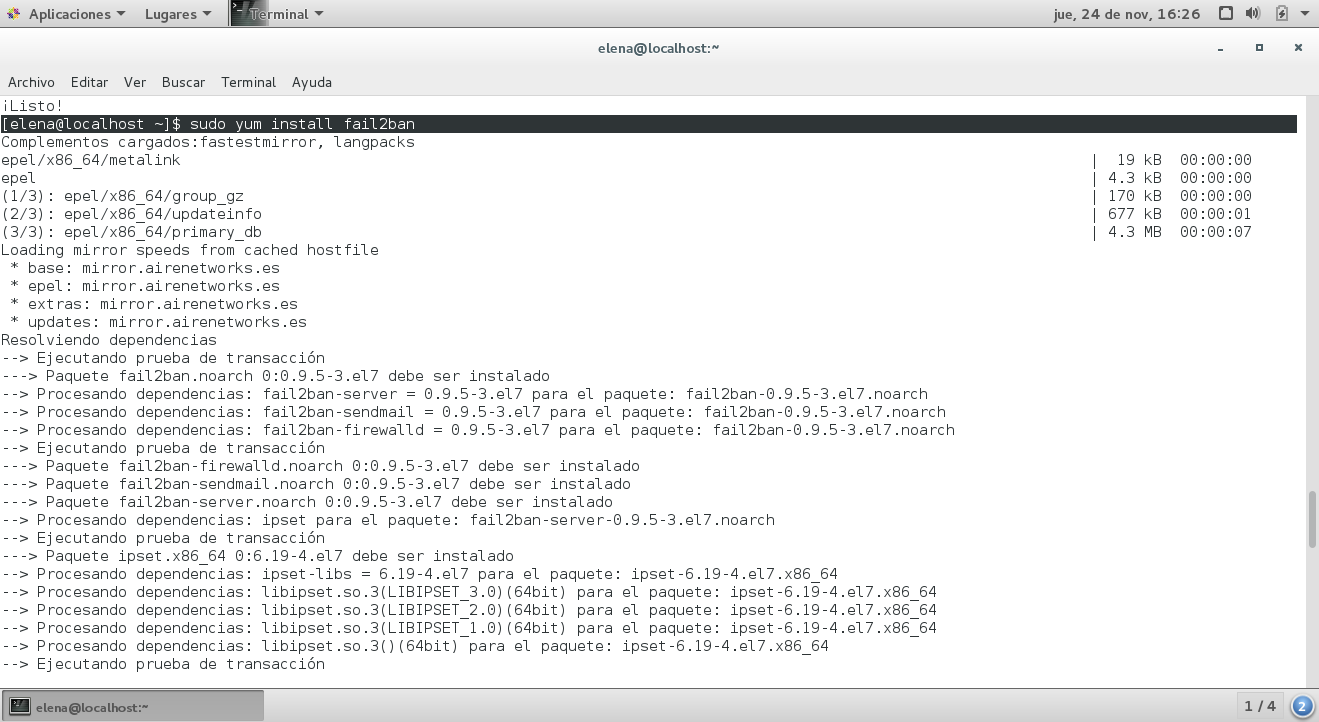
\includegraphics[width=15cm]{./img/opcional2b.png} 	
	\caption{CentOS, instalar fail2ban.} \label{fig:opcional2b}
\end{figure}

%----------------------------------------------------------------------------------------
%  Cuestión opcional 3
%----------------------------------------------------------------------------------------

%\section{Cuestión opcional 3: Instale el servicio y pruebe su funcionamiento.}


%----------------------------------------------------------------------------------------
%  Cuestión 9
%----------------------------------------------------------------------------------------

\section{Cuestión 9: Muestre los comandos que ha utilizado en Ubuntu Server y en CentOS (aunque en este último puede utilizar la GUI, en tal caso, realice capturas de pantalla). Compruebe que la instalación ha sido correcta.}

\begin{enumerate}
	\item Instalación en Ubuntu Server de LAMP
	
Primero vamos a instalar el servicio apache, para ello utilizamos el comando \texttt{sudo apt-get install apache2 apache2-utils} (figura \ref{fig:ejercicio9a}). Una vez instalado pasamos a configurarlo modificando el fichero \texttt{/etc/apache2/mods-enabled/dir.conf} dejandolo como se muestra en la figura \ref{fig:ejercicio9b}. Reiniciamos el servicio con \texttt{sudo service apache2 restart} (figura \ref{fig:ejercicio9c}) y comprobamos que funciona (figura \ref{fig:ejercicio9h}).\\
A continuación instalamos MySQL Server con \texttt{sudo apt-get install mysql-server libapache2-mod-auth-mysql php5-mysql} como se muestra en la figura \ref{fig:ejercicio9d}, continuamos la instalación con \texttt{sudo mysql\_install\_db} y con \texttt{sudo mysql\_secure\_installation} (figura \ref{fig:ejercicio9f}).\\
Finalmente instalamos php utilizando \texttt{sudo apt-get install php5 php5-mysql php-pear php5-gd  php5-mcrypt php5-curl} como se muestra en la figura \ref{fig:ejercicio9g}.\\
Para comprobar el funcionamiento de php y MySQL creamos dos scripts en php. El primero de ellos lo creamos con \texttt{sudo nano /var/www/html/phpinfo.php} y añadimos la línea ``<?php phpinfo(); ?>''. El segundo lo creamos con \texttt{sudo nano /var/www/html/phpmysql.php} y añadimos lo que se muestra en la figura \ref{fig:ejercicio9e}. Como se puede observar en la figura \ref{fig:ejercicio9i} funciona correctamente.

	
	\item Instalación en CentOS de LAMP
	
Primero instalamos el servicio apache con \texttt{yum install httpd} como se muestra en la figura \ref{fig:ejercicio9_1}. Una vez instalado iniciamos el servicio apache con \texttt{systemctl start httpd.service} (figura \ref{fig:ejercicio9_4}). Comprobamos que el servidor apache funciona tal y como se muestra en la figura \ref{fig:ejercicio9_3}. Por último habilitamos el servicio Apache para que se inicie al arrancar el sistema como se muestra en la figura \ref{fig:ejercicio9_4}.\\
A continuación instalamos MariaDB con \texttt{sudo yum install mariadb-server mariadb} (\ref{fig:ejercicio9_5}). Una vez completada la instalación iniciamos MariaDB con \texttt{sudo systemctl start mariadb}. Iniciamos la configuración con \texttt{sudo mysql\_secure\_installation}. Una vez finalizada habilitamos el servicio con \texttt{sudo systemctl enable mariadb.service} (figura \ref{fig:ejercicio9_6}).\\
Finalmente instalamos php utilizando \texttt{sudo yum install php php-mysql} (figura \ref{fig:ejercicio9_2}). Configuramos el firewall para permitir el acceso al servicio Apache como se muestra en la figura \ref{fig:ejercicio9_7}.\\
Vamos a probar que funciona, para ello al igual que en Ubuntu Server, creamos un script para php y otro para la conexión con MariaDB, tal y como se hizo en Ubuntu Server (figuras \ref{fig:ejercicio9_8} y \ref{fig:ejercicio9_9}).

\end{enumerate}


Para hacer la instalación en Ubuntu Server he seguido el tutorial \cite{LAMP} y para CentOS utilizo \cite{LAMPCentOS}.

\begin{figure}[H] 
	\centering
	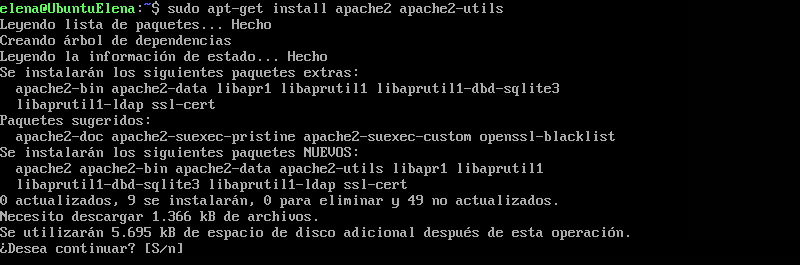
\includegraphics[width=15cm]{./img/ejercicio9a.png} 	
	\caption{Ubuntu Server, instalación de apache.} \label{fig:ejercicio9a}
\end{figure}


\begin{figure}[H] 
	\centering
	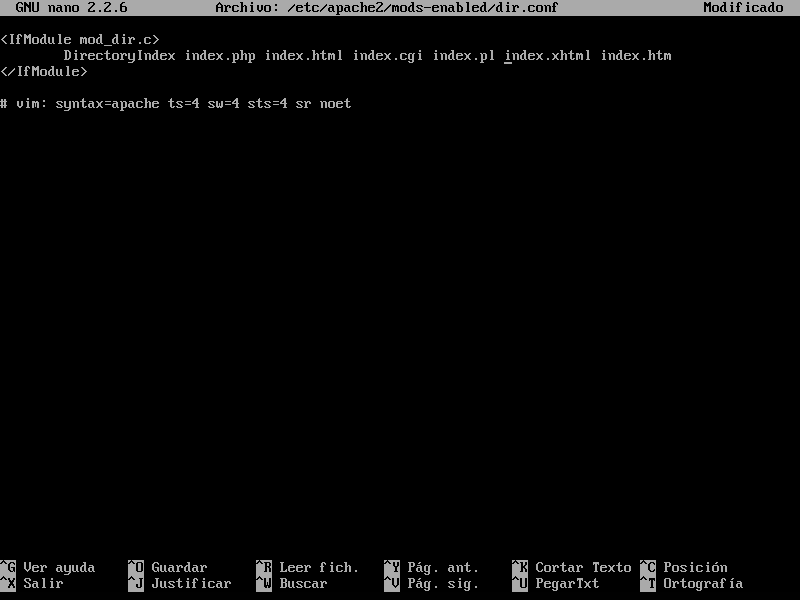
\includegraphics[width=15cm]{./img/ejercicio9b.png} 	
	\caption{Ubuntu Server, cambio configuración de apache.} \label{fig:ejercicio9b}
\end{figure}


\begin{figure}[H] 
	\centering
	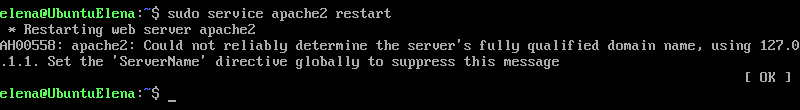
\includegraphics[width=15cm]{./img/ejercicio9c.png} 	
	\caption{Ubuntu Server, reinicio del servicio apache.} \label{fig:ejercicio9c}
\end{figure}


\begin{figure}[H] 
	\centering
	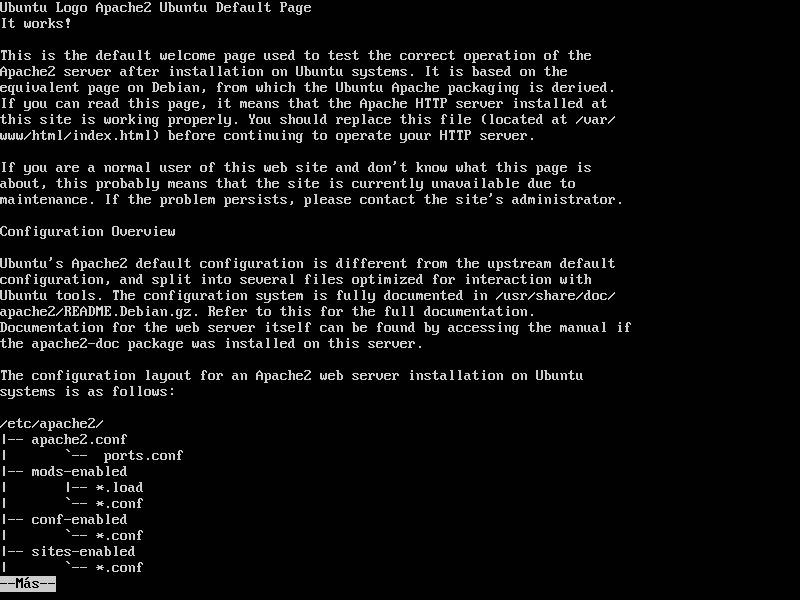
\includegraphics[width=15cm]{./img/ejercicio9h.png} 	
	\caption{Ubuntu Server, comprobación de funcionamiento de apache.} \label{fig:ejercicio9h}
\end{figure}

\begin{figure}[H] 
	\centering
	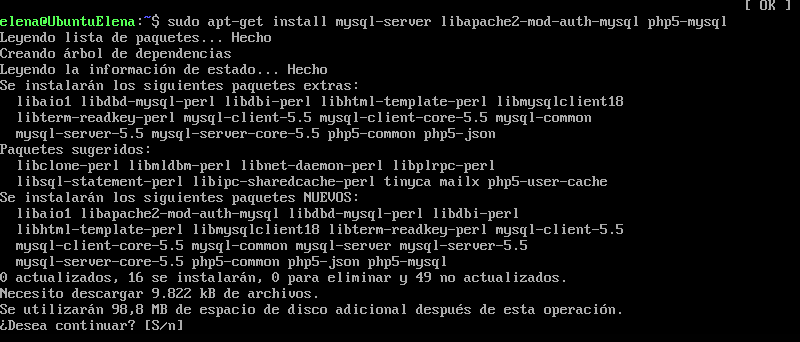
\includegraphics[width=15cm]{./img/ejercicio9d.png} 	
	\caption{Ubuntu Server, instalación de mysql.} \label{fig:ejercicio9d}
\end{figure}


\begin{figure}[H] 
	\centering
	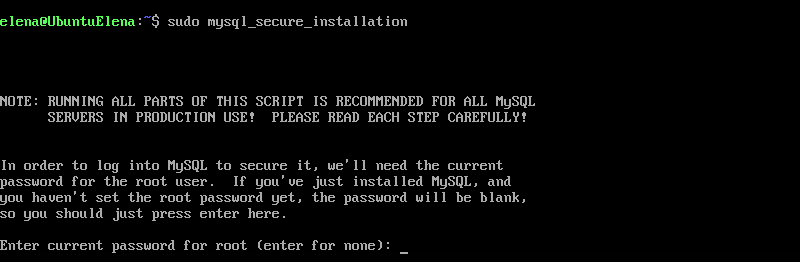
\includegraphics[width=15cm]{./img/ejercicio9f.png} 	
	\caption{Ubuntu Server, instalación de mysql.} \label{fig:ejercicio9f}
\end{figure}


\begin{figure}[H] 
	\centering
	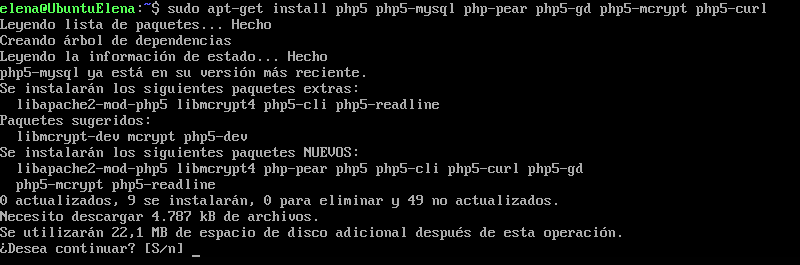
\includegraphics[width=15cm]{./img/ejercicio9g.png} 	
	\caption{Ubuntu Server, instalación de php.} \label{fig:ejercicio9g}
\end{figure}

\begin{figure}[H] 
	\centering
	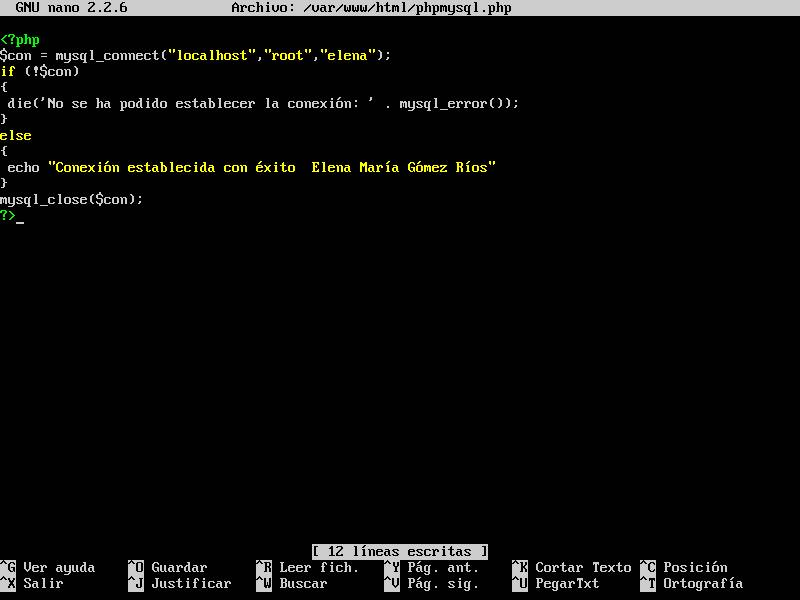
\includegraphics[width=15cm]{./img/ejercicio9e.png} 	
	\caption{Ubuntu Server, script de conexión a mysql.} \label{fig:ejercicio9e}
\end{figure}


\begin{figure}[H] 
	\centering
	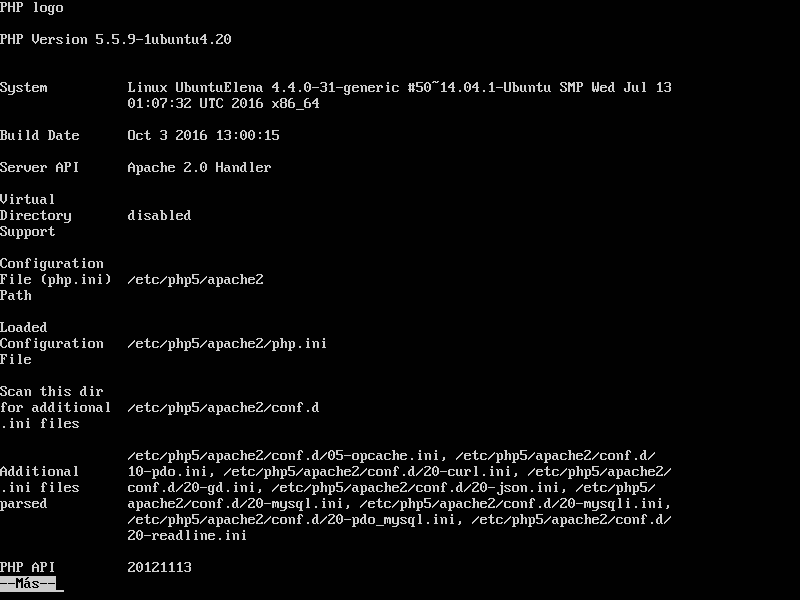
\includegraphics[width=15cm]{./img/ejercicio9i.png} 	
	\caption{Ubuntu Server, acceso a localhost/phpinfo.php.} \label{fig:ejercicio9i}
\end{figure}



\begin{figure}[H] 
	\centering
	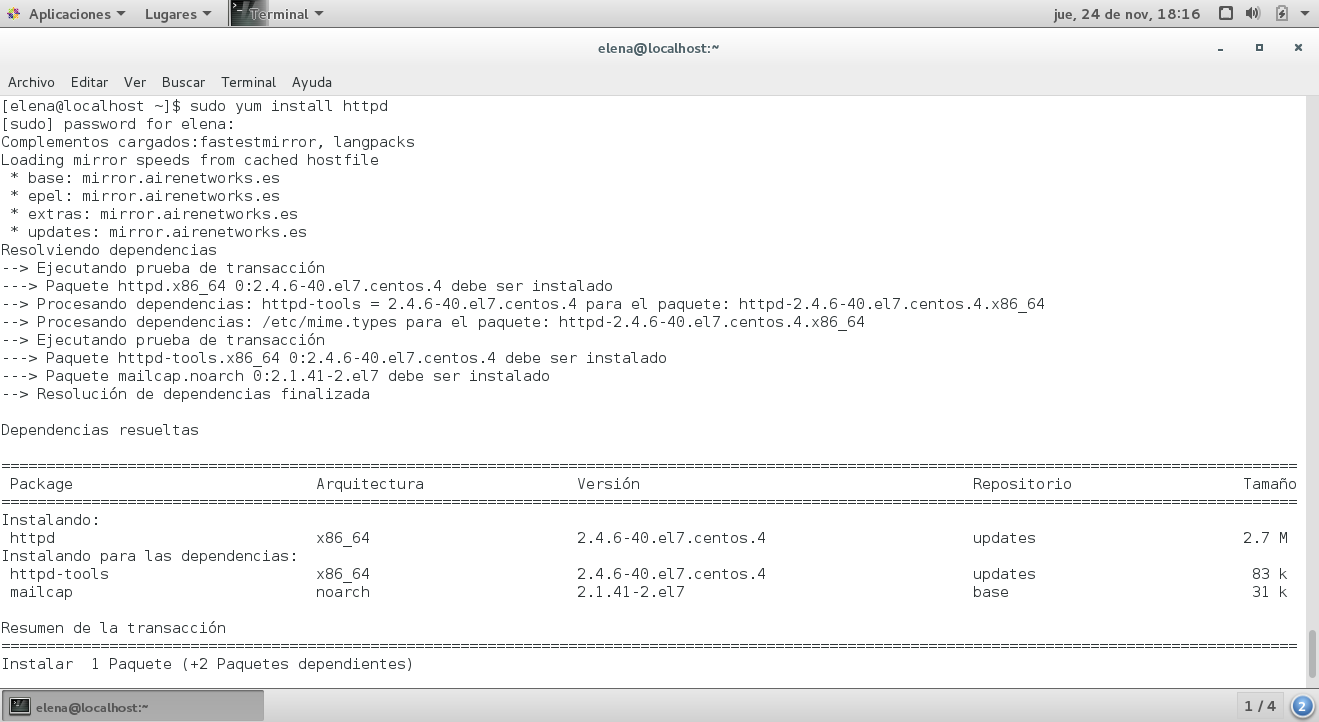
\includegraphics[width=15cm]{./img/ejercicio9_1.png} 	
	\caption{CentOS, instalación de apache.} \label{fig:ejercicio9_1}
\end{figure}


\begin{figure}[H] 
	\centering
	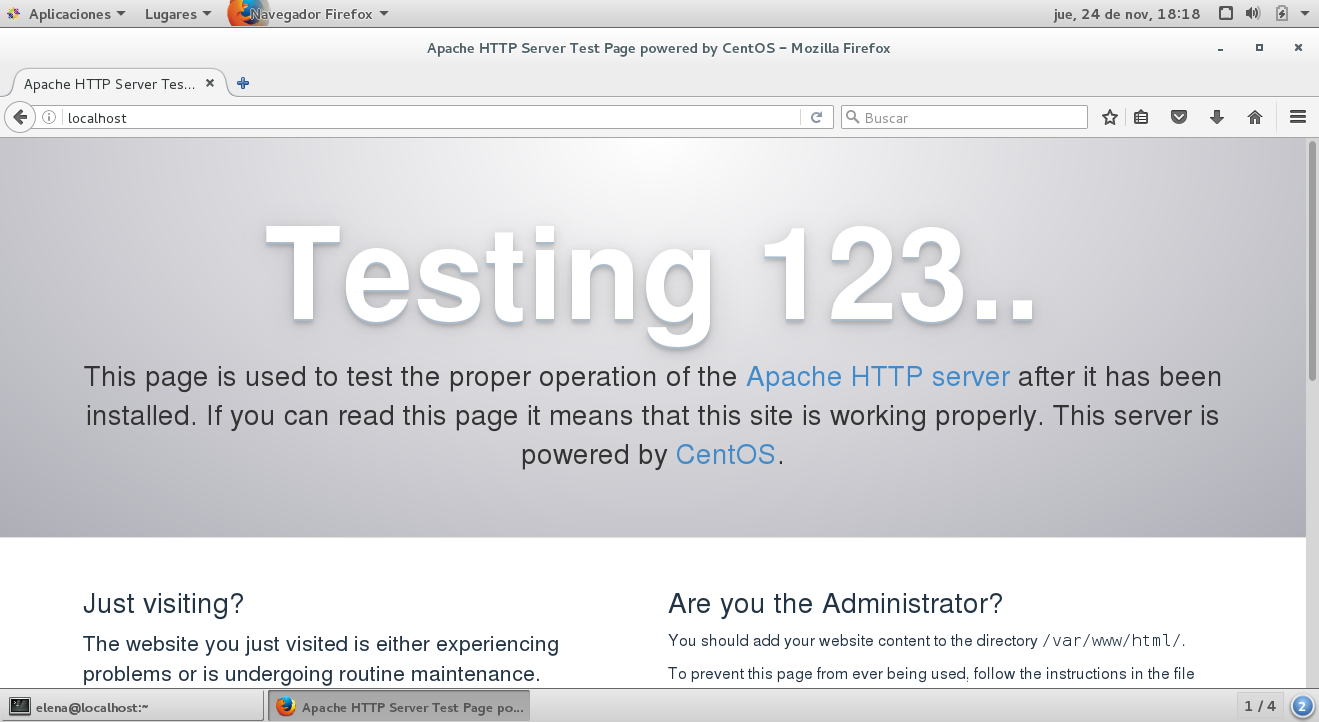
\includegraphics[width=15cm]{./img/ejercicio9_3.png} 	
	\caption{CentOS, pagina apache por defecto.} \label{fig:ejercicio9_3}
\end{figure}

\begin{figure}[H] 
	\centering
	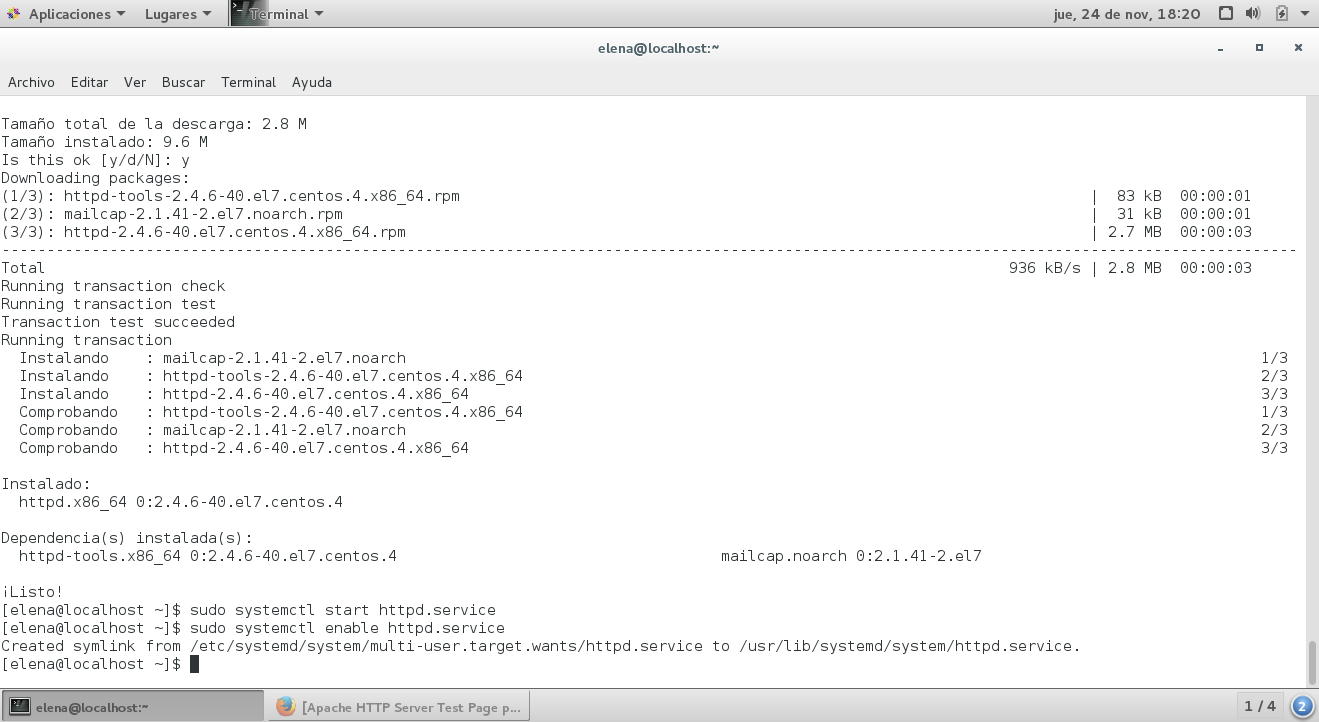
\includegraphics[width=15cm]{./img/ejercicio9_4.png} 	
	\caption{CentOS, inicio del servicio apache.} \label{fig:ejercicio9_4}
\end{figure}


\begin{figure}[H] 
	\centering
	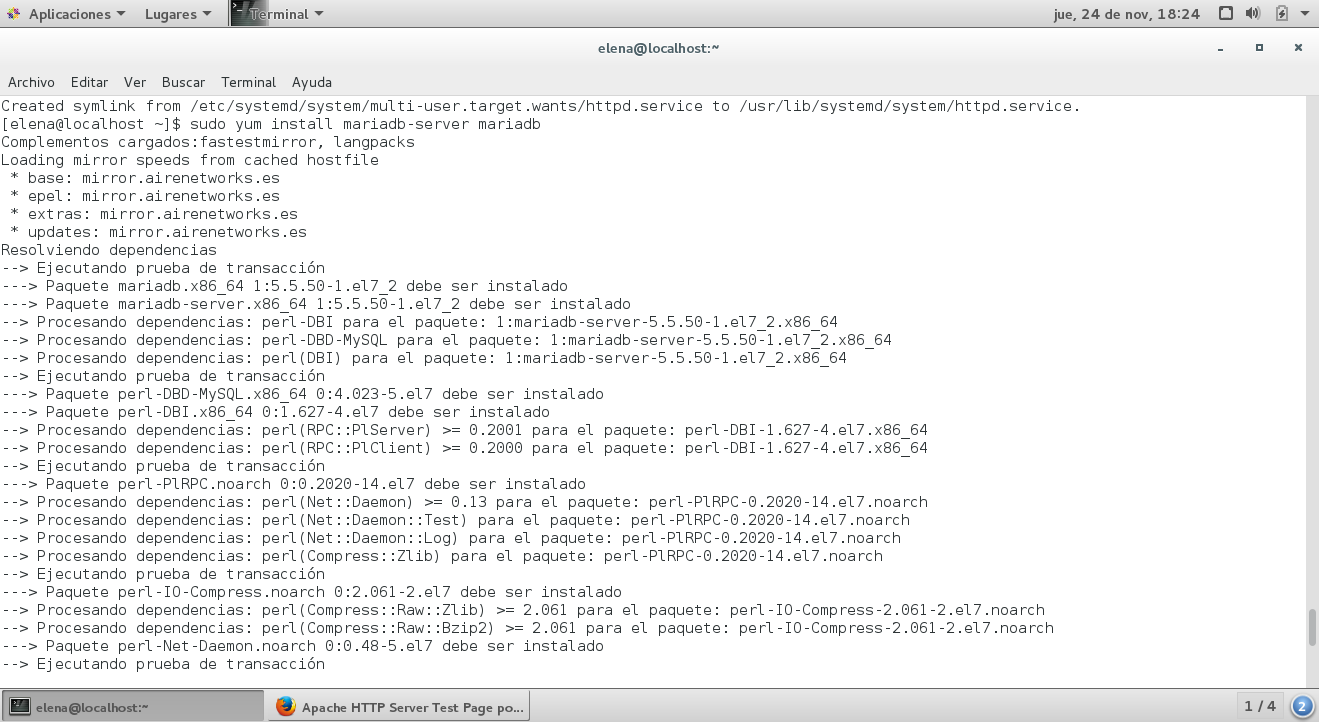
\includegraphics[width=15cm]{./img/ejercicio9_5.png} 	
	\caption{CentOS, instalación de mariadb.} \label{fig:ejercicio9_5}
\end{figure}


\begin{figure}[H] 
	\centering
	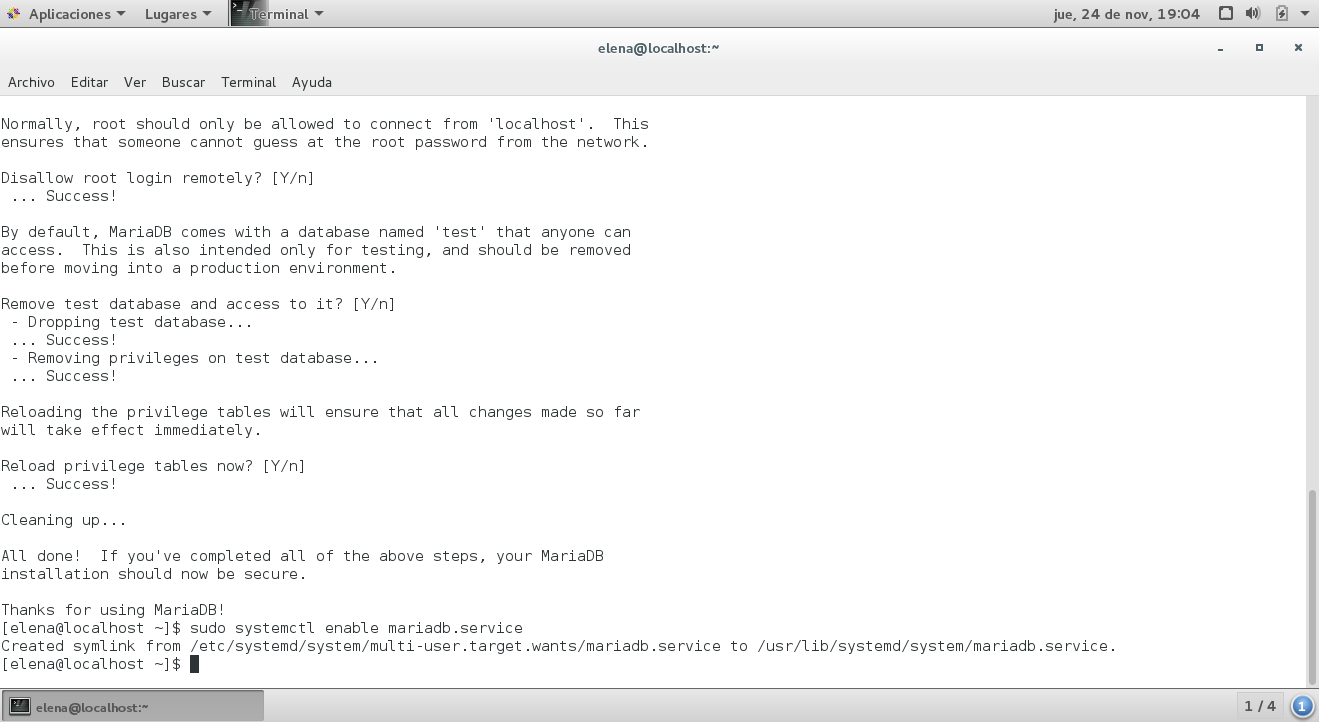
\includegraphics[width=15cm]{./img/ejercicio9_6.png} 	
	\caption{CentOS, configuración de mariadb.} \label{fig:ejercicio9_6}
\end{figure}


\begin{figure}[H] 
	\centering
	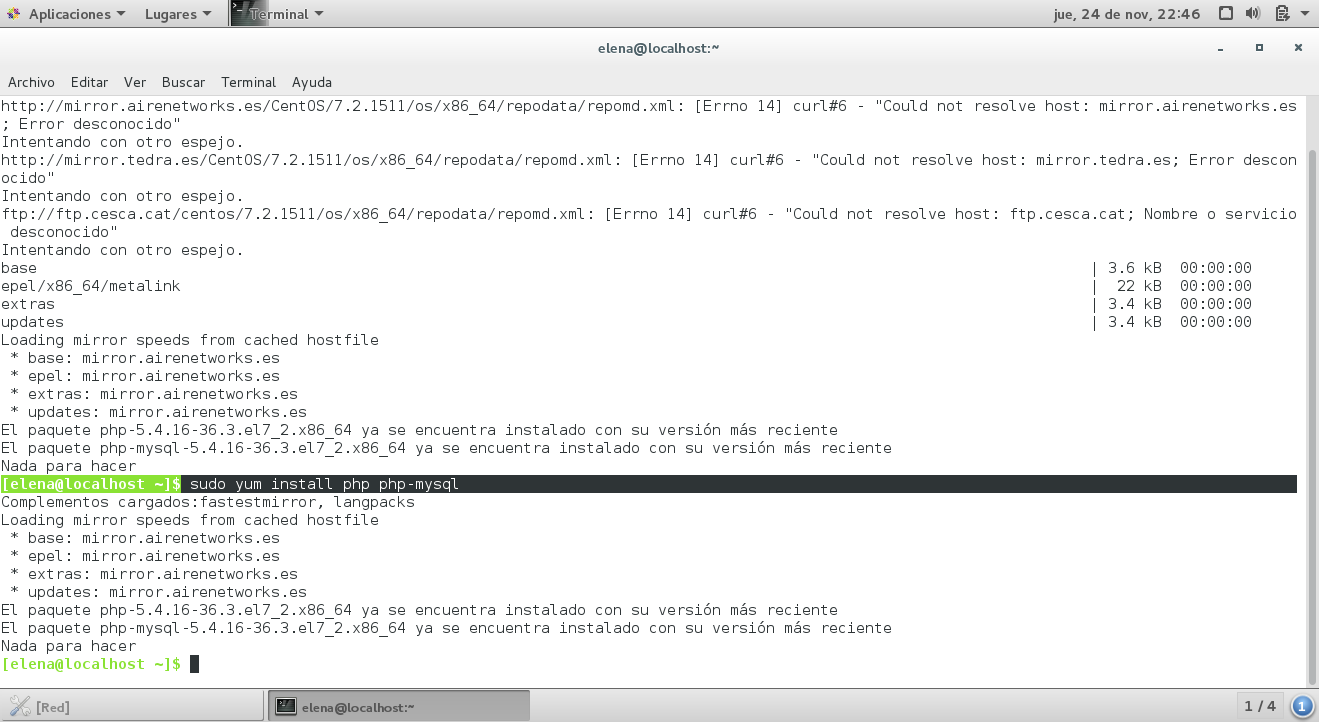
\includegraphics[width=15cm]{./img/ejercicio9_2.png} 	
	\caption{CentOS, instalación de php.} \label{fig:ejercicio9_2}
\end{figure}

\begin{figure}[H] 
	\centering
	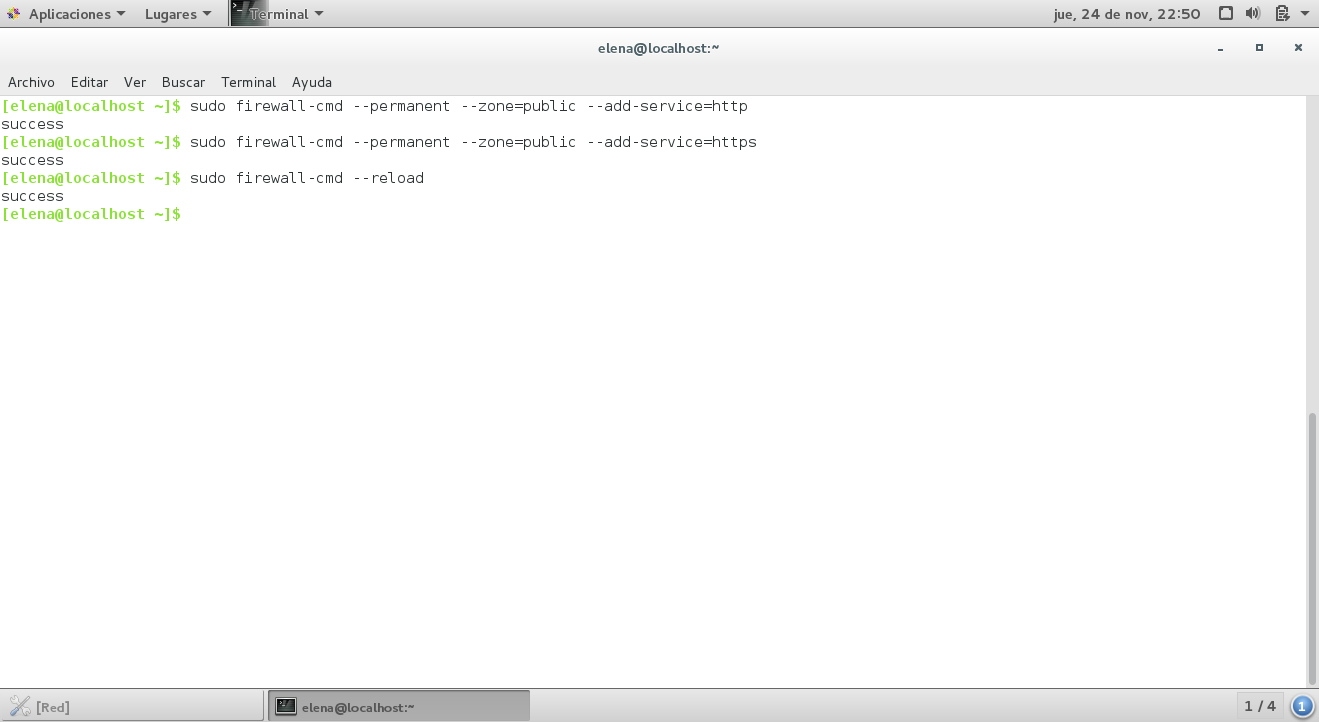
\includegraphics[width=15cm]{./img/ejercicio9_7.png} 	
	\caption{CentOS, configuración del firewall.} \label{fig:ejercicio9_7}
\end{figure}

\begin{figure}[H] 
	\centering
	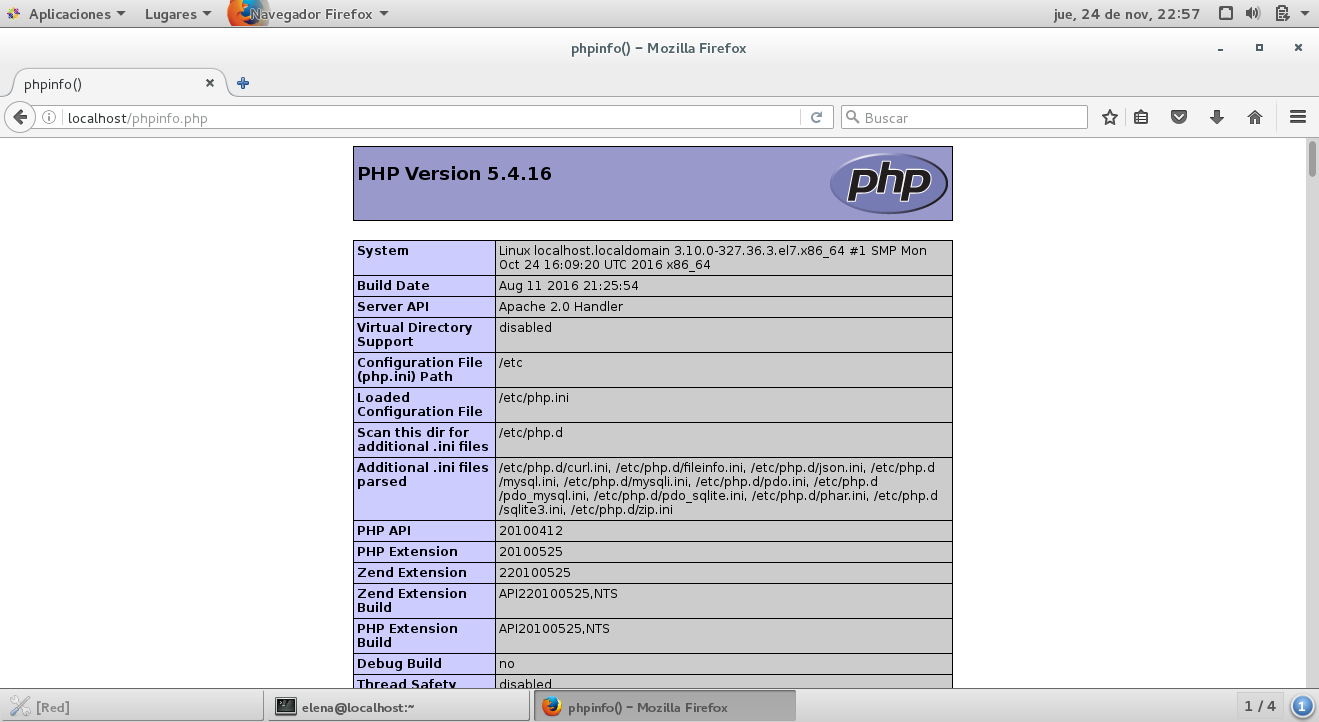
\includegraphics[width=15cm]{./img/ejercicio9_8.png} 	
	\caption{CentOS, comprobación de php.} \label{fig:ejercicio9_8}
\end{figure}

\begin{figure}[H] 
	\centering
	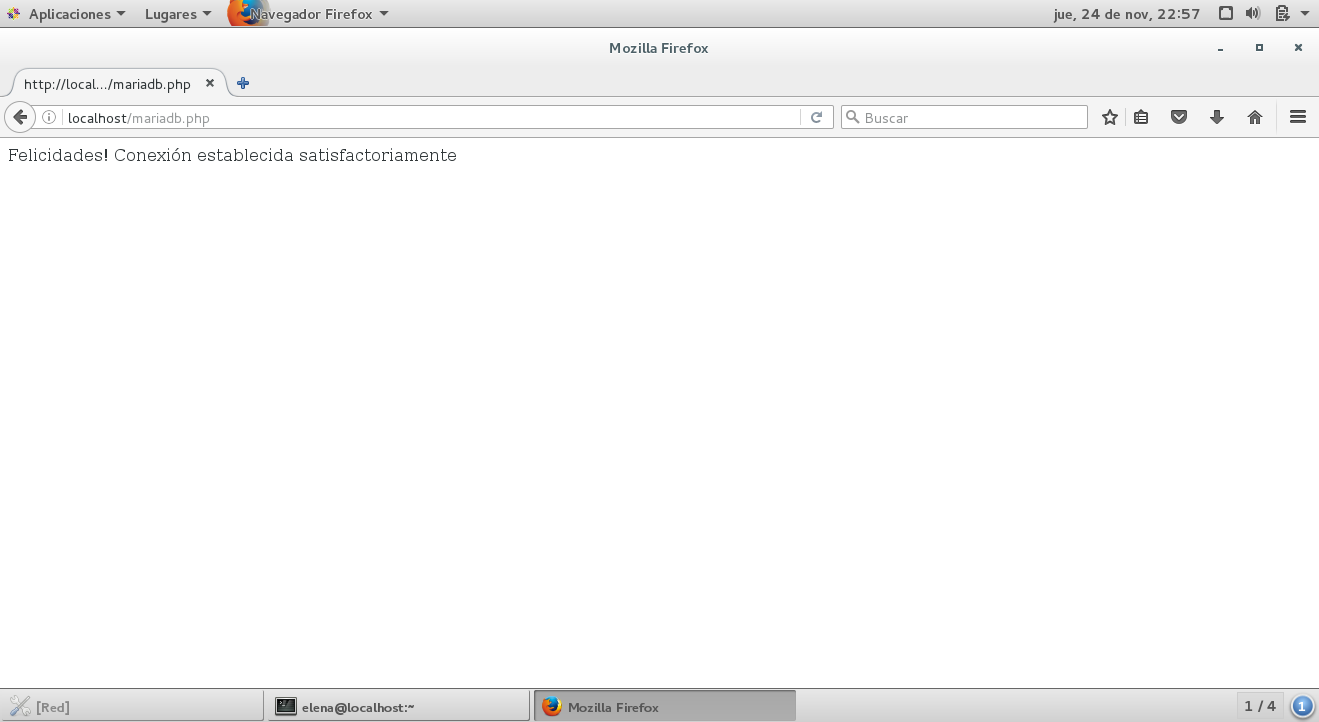
\includegraphics[width=15cm]{./img/ejercicio9_9.png} 	
	\caption{CentOS, comprobación de MariaDB.} \label{fig:ejercicio9_9}
\end{figure}




%----------------------------------------------------------------------------------------
%  Cuestión 10
%----------------------------------------------------------------------------------------

\section{Cuestión 10: Realice la instalación usando GUI o PowerShell y compruebe que el servicio está funcionando accediendo a la MV a través de la anfitriona.}


He instalado el servidor Web en Windows siguiendo los pasos del guión de prácticas, tal y como se puede ver en las figuras \ref{fig:ejercicio10_1}, \ref{fig:ejercicio10_2} y \ref{fig:ejercicio10_3}.
Para comprobar el correcto funcionamiento accedo al servidor Web desde Windows Server (figura \ref{fig:ejercicio10_4}) y CentOS (figura \ref{fig:ejercicio10_5}).

\begin{figure}[H] 
	\centering
	\includegraphics[width=15cm]{./img/ejercicio10_1.png} 	
	\caption{Windows, instalación del servidor Web (IIS).} \label{fig:ejercicio10_1}
\end{figure}

\begin{figure}[H] 
	\centering
	\includegraphics[width=15cm]{./img/ejercicio10_2.png} 	
	\caption{Windows, instalación del servidor Web (IIS).} \label{fig:ejercicio10_2}
\end{figure}

\begin{figure}[H] 
	\centering
	\includegraphics[width=15cm]{./img/ejercicio10_3.png} 	
	\caption{Windows, instalación del servidor Web (IIS).} \label{fig:ejercicio10_3}
\end{figure}

\begin{figure}[H] 
	\centering
	\includegraphics[width=15cm]{./img/ejercicio10_4.png} 	
	\caption{Windows, acceso al servidor Web (IIS).} \label{fig:ejercicio10_4}
\end{figure}

\begin{figure}[H] 
	\centering
	\includegraphics[width=15cm]{./img/ejercicio10_5.png} 	
	\caption{CentOS, acceso al servidor web de Windows.} \label{fig:ejercicio10_5}
\end{figure}

%----------------------------------------------------------------------------------------
%  Cuestión opcional 4
%----------------------------------------------------------------------------------------

%\section{Cuestión opcional 4: Realice la instalación de uno de estos dos “web containers” y pruebe su ejecución.}


%----------------------------------------------------------------------------------------
%  Cuestión opcional 5
%----------------------------------------------------------------------------------------

%\section{Cuestión opcional 5: Realice la instalación de MongoDB en alguna de sus máquinas virtuales. Cree una colección de documentos y haga una consulta sobre ellos. ( http://docs.mongodb.org/manual/installation/ )}


%----------------------------------------------------------------------------------------
%  Cuestión 11
%----------------------------------------------------------------------------------------

\section{Cuestión 11: Muestre un ejemplo http://fedoraproject.org/wiki/VMWare)}
Para la realización de este ejercicio he seguido el tutorial \cite{patch}. He creado un programa en c de prueba, y luego con patch, tal y como se muestra paso a paso en la figura \ref{fig:ejercicio11}, añado la línea con mi nombre.

\begin{figure}[H] 
	\centering
	\includegraphics[width=15cm]{./img/ejercicio11.png} 	
	\caption{CentOS, ejemplo de uso del comando patch.} \label{fig:ejercicio11}
\end{figure}



%----------------------------------------------------------------------------------------
%  Cuestión 12
%----------------------------------------------------------------------------------------

\section{Cuestión 12: Realice la instalación de esta aplicación y pruebe a modificar algún parámetro de algún servicio. Muestre las capturas de pantalla pertinentes así como el proceso de instalación.}

Instalo en CentOS la aplicación webmin siguiendo los pasos que se indican en \cite{webmin}.Primero realizamos la descarga del paquete y luego iniciamos la instalación con rpm, tal como se observa en las figuras \ref{fig:ejercicio12_1}, \ref{fig:ejercicio12_2} y \ref{fig:ejercicio12_3}.

Para comprobar que la instalación se ha realizado correctamente accedemos al panel de acceso de Webmin (figura  \ref{fig:ejercicio12_4}), y cambiamos algún parámetro, como por ejemplo la página de inicio del servidor web (figuras \ref{fig:ejercicio12_5}, \ref{fig:ejercicio12_6} y \ref{fig:ejercicio12_7}).


\begin{figure}[H] 
	\centering
	\includegraphics[width=15cm]{./img/ejercicio12_1.png} 	
	\caption{CentOS, Instalación de webmin.} \label{fig:ejercicio12_1}
\end{figure}

\begin{figure}[H] 
	\centering
	\includegraphics[width=15cm]{./img/ejercicio12_2.png} 	
	\caption{CentOS, Instalación de webmin.} \label{fig:ejercicio12_2}
\end{figure}

\begin{figure}[H] 
	\centering
	\includegraphics[width=15cm]{./img/ejercicio12_3.png} 	
	\caption{CentOS, Instalación de webmin.} \label{fig:ejercicio12_3}
\end{figure}

\begin{figure}[H] 
	\centering
	\includegraphics[width=15cm]{./img/ejercicio12_4.png} 	
	\caption{CentOS, panel de acceso de webmin.} \label{fig:ejercicio12_4}
\end{figure}

\begin{figure}[H] 
	\centering
	\includegraphics[width=15cm]{./img/ejercicio12_5.png} 	
	\caption{CentOS, panel de configuración de webmin.} \label{fig:ejercicio12_5}
\end{figure}

\begin{figure}[H] 
	\centering
	\includegraphics[width=15cm]{./img/ejercicio12_6.png} 	
	\caption{CentOS, panel de configuración de webmin.} \label{fig:ejercicio12_6}
\end{figure}

\begin{figure}[H] 
	\centering
	\includegraphics[width=15cm]{./img/ejercicio12_7.png} 	
	\caption{CentOS, cambio de página de inicio.} \label{fig:ejercicio12_7}
\end{figure}



%----------------------------------------------------------------------------------------
%  Cuestión 13
%----------------------------------------------------------------------------------------

\section{Cuestión 13 : Instale phpMyAdmin, indique cómo lo ha realizado y muestre algunas capturas de pantalla. Configure PHP para poder importar BDs de hasta 25MiB (en vez de los 8 MiB de límite por defecto). Indique cómo ha realizado el proceso y muestre capturas de pantalla.}

Primero instalo phpMyAdmin con \texttt{sudo yum install phpmyadmin} (figura \ref{fig:ejercicio13_1}). Para que funcione hace falta reiniciar el servicio apache con \texttt{sudo systemctl restart httpd.service}, y ya podemos acceder a phpMyAdmin tal y como se muestra en la figura  \ref{fig:ejercicio13_2}.

Ahora vamos a realizar la configuración para poder importar bases de datos de hasta 25 MiB, para ello modificamos en el archivo \texttt{/etc/php.ini} las variables ``post\_max\_size'' y ``upload\_max\_filesize'' que hacen referencia al tamaño máximo de datos permitidos (figuras \ref{fig:ejercicio13_3} y \ref{fig:ejercicio13_4}). Como se puede observar en la figura \ref{fig:ejercicio13_5} el cambio se ha realizado correctamente.




\begin{figure}[H] 
	\centering
	\includegraphics[width=15cm]{./img/ejercicio13_1.png} 	
	\caption{CentOS, instalación de phpMyAdmin.} \label{fig:ejercicio13_1}
\end{figure}

\begin{figure}[H] 
	\centering
	\includegraphics[width=15cm]{./img/ejercicio13_2.png} 	
	\caption{CentOS, phpMyAdmin.} \label{fig:ejercicio13_2}
\end{figure}

\begin{figure}[H] 
	\centering
	\includegraphics[width=15cm]{./img/ejercicio13_3.png} 	
	\caption{CentOS, cambio en la configuración de phpMyAdmin.} \label{fig:ejercicio13_3}
\end{figure}

\begin{figure}[H] 
	\centering
	\includegraphics[width=15cm]{./img/ejercicio13_4.png} 	
	\caption{CentOS, cambio en la configuración de phpMyAdmin.} \label{fig:ejercicio13_4}
\end{figure}

\begin{figure}[H] 
	\centering
	\includegraphics[width=15cm]{./img/ejercicio13_5.png} 	
	\caption{CentOS, tamaño de 25MiB en phpMyAdmin.} \label{fig:ejercicio13_5}
\end{figure}



%----------------------------------------------------------------------------------------
%  Cuestión 14
%----------------------------------------------------------------------------------------

\section{Cuestión 14: Viste al menos una de las webs de los software mencionados y pruebe las demos que ofrecen realizando capturas de pantalla y comentando qué está realizando.}
Vamos a probar el editor de host web \texttt{Parallel Plesk}, en la página de demostración vemos un resumen del servidor web, como se aprecia en la figura \ref{fig:ejercicio14_1}. Accedemos al apartado de clientes (figura \ref{fig:ejercicio14_2}) y vemos que cuenta con una amplia variedad de opciones y de control sobre los clientes. Creamos un cliente y resulta muy fácil e intuitivo. También miramos la gestión de los dominios del servidor (figura \ref{fig:ejercicio14_3}), donde aparece el dominio que creamos durante el alta de un nuevo cliente. Plesk cuenta también con una amplia variedad de herramientas y opciones como se muestra en la figura \ref{fig:ejercicio14_4}. Algunas de las opciones más útiles son las copias de seguridad del sevidor (figura \ref{fig:ejercicio14_5}) y la seguridad del servidor, expectablemente miramos los certificados SSL/TLS (figura \ref{fig:ejercicio14_6}).\\

Como se puede observar el uso de \texttt{Parallel Plesk} es bastante fácil e intuitivo, haciendo fácil la administración del servidor sin tener unos conocimientos amplios sobre el tema.


\begin{figure}[H] 
	\centering
	\includegraphics[width=15cm]{./img/ejercicio14_1.png} 	
	\caption{CentOS,Plesk pantalla de inicio de la demo} \label{fig:ejercicio14_1}
\end{figure}

\begin{figure}[H] 
	\centering
	\includegraphics[width=15cm]{./img/ejercicio14_2.png} 	
	\caption{CentOS, Plesk pantalla de clientes de la demo} \label{fig:ejercicio14_2}
\end{figure}

\begin{figure}[H] 
	\centering
	\includegraphics[width=15cm]{./img/ejercicio14_3.png} 	
	\caption{CentOS, Plesk pantalla de dominios de la demo} \label{fig:ejercicio14_3}
\end{figure}

\begin{figure}[H] 
	\centering
	\includegraphics[width=15cm]{./img/ejercicio14_4.png} 	
	\caption{CentOS, Plesk pantalla de herramientas de la demo} \label{fig:ejercicio14_4}
\end{figure}

\begin{figure}[H] 
	\centering
	\includegraphics[width=15cm]{./img/ejercicio14_5.png} 	
	\caption{CentOS, Plesk pantalla de copias de seguridad de la demo} \label{fig:ejercicio14_5}
\end{figure}

\begin{figure}[H] 
	\centering
	\includegraphics[width=15cm]{./img/ejercicio14_6.png} 	
	\caption{CentOS,Plesk pantalla de certificado de la demo} \label{fig:ejercicio14_6}
\end{figure}



%----------------------------------------------------------------------------------------
%  Cuestión 15
%----------------------------------------------------------------------------------------

\section{Cuestión 15 :}

\subsection{a) Ejecute los ejemplos de find, grep }
Ejecutamos los comandos como se ve en la figura \ref{fig:ejercicio15a}.

\begin{figure}[H] 
	\centering
	\includegraphics[width=15cm]{./img/ejercicio15a.png} 	
	\caption{CentOS, ejecución de comandos find y grep} \label{fig:ejercicio15a}
\end{figure}


\subsection{b) Escriba el script que haga uso de sed para cambiar la configuración de ssh y reiniciar el servicio. }
Hemos creado un script llamado \texttt{ejercicio15b.sh} para cambiar los puertos del servicio ssh cuyo contenido se puede ver en la figura \ref{fig:ejercicio15b_1}. Le damos permisos de ejecución al script y lo ejecutamos (figura \ref{fig:ejercicio15b_2}), y como se puede observar en las figuras los cambios se hacen correctamente (figuras \ref{fig:ejercicio15b_3} y \ref{fig:ejercicio15b_4}).


\begin{figure}[H] 
	\centering
	\includegraphics[width=15cm]{./img/ejercicio15b_1.png} 	
	\caption{CentOS, script para cambiar puertos del ssh.} \label{fig:ejercicio15b_1}
\end{figure}

\begin{figure}[H] 
	\centering
	\includegraphics[width=15cm]{./img/ejercicio15b_2.png} 	
	\caption{CentOS, ejecución del script para cambiar puertos del ssh.} \label{fig:ejercicio15b_2}
\end{figure}

\begin{figure}[H] 
	\centering
	\includegraphics[width=15cm]{./img/ejercicio15b_3.png} 	
	\caption{CentOS, configuración antes de ejecutar el script.} \label{fig:ejercicio15b_3}
\end{figure}

\begin{figure}[H] 
	\centering
	\includegraphics[width=15cm]{./img/ejercicio15b_4.png} 	
	\caption{CentOS, configuración después de ejecutar el script.} \label{fig:ejercicio15b_4}
\end{figure}

\subsection{c) Muestre un ejemplo de uso para awk.}
Para los ejemplos de uso del comando \texttt{awk} hemos seguido el tutorial \cite{awk}.\\

Primero creo un archivo de prueba (figura \ref{fig:ejercicio15c_1}) sobre el que poder utilizar \texttt{awk} (figura \ref{fig:ejercicio15c_2}).

\begin{figure}[H] 
	\centering
	\includegraphics[width=15cm]{./img/ejercicio15c_1.png} 	
	\caption{CentOS, fichero prueba awk.} \label{fig:ejercicio15c_1}
\end{figure}

\begin{figure}[H] 
	\centering
	\includegraphics[width=15cm]{./img/ejercicio15c_2.png} 	
	\caption{CentOS, ejemplos de uso de awk.} \label{fig:ejercicio15c_2}
\end{figure}


%----------------------------------------------------------------------------------------
%  Cuestión 16
%----------------------------------------------------------------------------------------

\section{Cuestión 16 : Escriba el script para cambiar el acceso a ssh usando PHP o Python.}



%----------------------------------------------------------------------------------------
%  Cuestión 17
%----------------------------------------------------------------------------------------

\section{Cuestión 17 : Abra una consola de Powershell y pruebe a parar un programa en ejecución (p.ej), realice capturas de pantalla y comente lo que muestra.}
Hemos utilizado \texttt{Powershell} para parar Internet Explorer, para ello primero listamos todos los procesos del sistema con el comando \texttt{Get-Process} como se muestra en la figura \ref{fig:ejercicio17_1}. Una vez que conocemos el ID del proceso que queremos parar introducimos el comando \texttt{Stop-Process -ID <ID>} como se muestra en la figura \ref{fig:ejercicio17_2}


\begin{figure}[H] 
	\centering
	\includegraphics[width=15cm]{./img/ejercicio17_1.png} 	
	\caption{Windows, listado de procesos.} \label{fig:ejercicio17_1}
\end{figure}

\begin{figure}[H] 
	\centering
	\includegraphics[width=15cm]{./img/ejercicio17_2.png} 	
	\caption{Windows, terminación del proceso IExplorer.} \label{fig:ejercicio17_2}
\end{figure}

%------------------------------------------------

\section{Problemas}
No he podido hacer las pruebas desde la máquina anfitrión hacia las máquinas virtuales porque tengo un problema con los puertos en mi ordenador que no consigo arreglar, y para poder acceder desde la máquina anfitrión hasta las máquinas virtuales hace falta redirigir los puertos. Por lo tanto todas las pruebas las he hecho entre máquinas virtuales.


%------------------------------------------------

\bibliography{citas} %archivo citas.bib que contiene las entradas 
\bibliographystyle{plain} % hay varias formas de citar

\end{document}
